\documentclass[a4paper,12pt]{scrartcl} % the percent sign is used for comments.
\usepackage[margin=3cm]{geometry} % sets the borders to 3cm each
\usepackage[english]{babel}     %defines language for spacing
\usepackage[utf8]{inputenc}   % allows entering special characters
\usepackage[T1]{fontenc}        % sets font to T1 and allows umlaute
\usepackage{lmodern}            % improves font display in PDFs
\usepackage{microtype}          % improves spacing when using lmodern
\usepackage{amsmath,amsfonts,amssymb}   % allows particular math environments
\usepackage{graphicx}           % allows using graphics
\usepackage{booktabs}           %allows creating professional tables with commands like \toprule
\usepackage{csquotes}           % better use of quotation marks, makes them context-sensitive
%\usepackage{longtable}          % allows for Table over more than one page
%\usepackage{sidewaystable}          % allows creating landscape tables
\usepackage[labelfont=bf,format=hang]{caption} % more powerful caption of figures and tables; The language for the caption label like Figure is boldface (bf). The language is taken from the babel package, i.e. Abbildung if german instead of english.

\usepackage{setspace}           % allows for \onehalfspacing and \doublespacing to set linespacing
\usepackage{epstopdf}           % allows using eps-file with pdflatex
\usepackage{textcomp}           % adds more symbols
%\usepackage{indentfirst}       % use if you want to indent first row
\usepackage[hyphens]{url}       % breaks overlong URLs (needs to be before biblatex)

%%%% define the usage of BibLaTeX for citations and bibliographies
\usepackage[%
citestyle=authoryear-comp,%use compressed author-year citation
bibstyle=JME,% use JME-style; change to JME_sentencecase to have all titles converted to lowercase letters
maxbibnames=5,% %maximum number of names printed in bibliography before truncation with ``et al.'' is used
minbibnames=1, % number of authors displayed if truncation happens
maxnames=4,% maximum number of names printed in citation before et al. is used
minnames=1,% number of authors displayed if truncation happens
datezeros=false,% no leading 0 if dates are printed
date=long,%
isbn=false,% show no ISBNs in bibliography (applies only if not a mandatory field)
url=false,% show no urls in bibliography (applies only if not a mandatory field)
doi=false, % show no dois in bibliography (applies only if not a mandatory field)
eprint=false, %show no eprint-field in bibliography (applies only if not a mandatory field)
backend=biber %use biber as the backend; backend=bibtex is less powerful, but easier to install
]{biblatex}

\addbibresource{../mybibfile.bib} % defines the name of the .bib-file	



\usepackage[pdfpagelabels=true,plainpages=false,pdftex,bookmarksnumbered=false,bookmarksopen=true]{hyperref}%plainpage and pdfpagelabels allows for correct figure links when using different page numberings
% bookmarksnumbered=false shuts off TOC numbers in TOC of PDF
% bookmarksopen=true opens TOC in Abobe Reader on the left


\hypersetup{
pdfproducer = {LaTeX},
colorlinks,
linkcolor=black,
filecolor=yellow,
urlcolor=blue,
citecolor=black,
pdftitle ={Title of the thesis},
pdfsubject ={Thesis},
pdfauthor = {Your Name },
pdfkeywords = {Some keywords}
pdfcreator={pdfLaTex}}



\usepackage[%
nonumberlist, %switch of displaying page numbers
acronym,      %creates List of Abbreviations
%toc,          %triggers entry into table of content
%section      %defines the level where the TOC entry appears
]{glossaries} % used to create list of symbols and abbreviations; one of the few packages to be defined after hyperref

\newglossary[slg]{symbolslist}{syi}{syg}{List of Symbols} %defines a new list called symbolslist for the List of symbols

\makeglossaries %need for sorting of entries to list of symbols and abbreviations; must be defined after all \newglossary commands

%% define terms for List of Symbols; entries only appear if they have been referenced in the main document  using either \gls{} or \glsadd{}

\newglossaryentry{symb:pi}{%
    name={\ensuremath{\pi}}, %define symbol; the \ensuremath ensures the symbol can be used inside and outside math environments
    description={ratio of circumference of circle to its diameter}, % the description that appears in the list of symbols
    sort=symbolpi, % key for sorting the symbols
    type=symbolslist % specifies that the entry belongs to the symbolslist-list and not the default (acronym) list
    }

\newglossaryentry{symb:i}{name={\ensuremath{i}},description={square root of $-1$},sort=symboli,type=symbolslist}
\newglossaryentry{symb:e}{name={\ensuremath{e}},description={Euler number},sort=symbole,type=symbolslist}

\newacronym{acro:OLS}{OLS}{Ordinary Least Squares}%defines the acronym OLS
\glsadd{acro:OLS} % add the acronym to the list of abbreviations, regardless of whether it has been used in the document

\onehalfspacing

% ________________ Set up the document ______________________%

\pagestyle{plain}          % empty header, page number in the middle of the footer
\newcommand{\bs}{\boldsymbol}  % shortcut to generate bold symbols in math environments
\setcounter{tocdepth}{3}   % The Table of contents is three levels deep, i.e. down to subsubsections.

% ________________ Defines command \ScaleIfNeeded that scales Figures to width of the page if they are larger ______________________%

\makeatletter
\def\ScaleIfNeeded{%
\ifdim\Gin@nat@width>\linewidth
\linewidth
\else
\Gin@nat@width
\fi
}
\makeatother


\begin{document}

% ________________ Title Page ______________________%



\pagenumbering{roman}   % Roman numbering

\begin{titlepage}

\thispagestyle{empty}   % no number on titlepage
%%%% to be deleted, only for information purposes

%%%%%


\begin{center}
\vspace*{2.cm}
{\textbf{  \Huge Practicing Dynare 4.5.6}} \\
\vspace*{2cm}
Francisco Barillas\\
New York University,Dept. of Economics\\
\vspace{0.5cm}
Anmol Bhandari\\
New York University,Dept. of Economics\\
\vspace{0.5cm}
Riccardo Colacito\\
University of North Carolina,Dept. of Finance\\
\vspace{0.5cm}
Sagiri Kitao\\
University of Southern California,FBE Deptartment\\
\vspace{0.5cm}
Christian Matthes\\
New York University,Dept. of Economics\\
\vspace{0.5cm}
Thomas J. Sargent\\
New York University,Dept. of Economics\\
\vspace{0.5cm}
Yongseok Shin\\
Washington University,Dept. of Economics
\end{center}


\vfill
\begin{flushright}
   \emph{Updated by:} \\
   \emph{Wenli Xu} \\
   \emph{Anhui University, School of Economics}\\
    \emph{CIMERS}\\
    \emph{March 10,2019}\\
\end{flushright}


\end{titlepage}

\clearpage                % forces a new page and setting of current float objects stored by Latex



% ________________ Table of Contents/Figures/Tables ______________________%

\tableofcontents
\clearpage
\listoffigures
\clearpage
\listoftables
\clearpage


% ________________ Main Matter ______________________%

\pagenumbering{arabic}      % Arabic Numbering
\setcounter{page}{1}        % Start Numbering at 1

\section{Introduction}

This paper describes nine examples or types of examples that illustrate how Dynare can approximate the solutions of dynamic rational expectations models, simulate them, and estimate them by maximum likelihood and Bayesian methods. Section 2 approximates and estimates a one-sector stochastic growth model. Section 3 approximates and estimates a two-country stochastic growth model. Section 4 follows chapter 11 of Ljungqvist and Sargent (2004) in studying the effects of foreseen fiscal policy in a non-stochastic growth model. Section 5 updates and extends these examples to correspond to chapter 11 of Ljungqvist and Sargent (20XX). Section 6 estimates a rational expectations model of hyperinflation originally formulated by Sargent (1977). Section 7 solves and estimates the permanent income model of Hall (1988). This application is interesting, among other reasons, for the way that it illustrates how Dynare can implement the ‘diffuse Kalman filter’ needed in situations in which an initial endogenous state variable is unknown and the model has a unit root. Section 8 solves and estimates the Ryoo and Rosen (2004) rational expectations model of a market for engineers. Section 9 estimates a model of consumption growth proposed by Bansal and Yaron (2004). Section 10 solves and estimates the Hansen, Sargent, and Tallarini (1999) model of robust permanent income and pricing. Section 11 solves and estimates the Bansal and Yaron (2004) of asset prices and long-run risk in consumption and dividends. Appendix A tells how the reader can obtain the file examples.zip that contain the *.mod and data files that we used to generate these examples.

Some of our examples bear eloquent witness to the technological improvements brought by Dynare. For example, the maximum likelihood estimates in Sargent (1977) and Hansen, Sargent, and Tallarini (1999) were time-consuming and painful to obtain originally. Dynare has reduced the time and the pain.

\section{The Neoclassical growth model} \label{sec:Section1}


\subsection{The model}

We study a widely used stochastic neoclassical growth model with leisure (see, for example, Cooley and Prescott
(1995)). A representative household’s problem is
$$\underbrace{max}_{c_t,l_t}~~E_0\sum_{t=1}^{\infty}\beta^{t-1}\frac{(c_t^\theta(1-l_t)^{1-\theta})^{1-\tau}}{1-\tau}$$

subject to the resource constraint
\begin{equation}\label{1}
  c_t+i_t=e^{z_t}k_t^{\alpha}l_t^{1-\alpha}
\end{equation}
the law of motion for capital
\begin{equation}\label{2}
  k_{t+1}=i_i+(1-\delta)k_t
\end{equation}
and the stochastic process for productivity
\begin{equation}\label{3}
   z_t=\rho z_{t-1}+s_t\epsilon_t
\end{equation}
with~$\epsilon_t~\sim ~N(0,\sigma^2).$

The system of equations characterizing an equilibrium is comprised of equations (1), (2) and (3), the Euler intertemporal condition
\begin{equation}\label{4}
   \frac{c_t^\theta(1-l_t)^{1-\theta})^{1-\tau}}{c_t}=\beta E_t\lgroup\frac{c_{t+1}^\theta(1-l_{t+1})^{1-\theta})^{1-\tau}}{c_{t+1}}(1+\alpha e^{z_t}k_t^{alpha-1}l_t^{\alpha}-\delta)\rgroup
\end{equation}
and an optimality condition for supply of labor
\begin{equation}\label{5}
   \frac{1-\theta}{\theta}\frac{c_t}{1-l_t}=(1-\alpha)e^{z_t}k_t^{\alpha}l_t^{-\alpha}
\end{equation}
Use (1) and (2) to get
\begin{equation}\label{6}
   k_{t+1}=e^{z_t}k_t^{\alpha}l_t^{1-\alpha}-c_t+(1-\delta)k_t
\end{equation}

An equilibrium is characterized by a system of four equations (3), (4), (5) and (6).

\subsection{Calibration and approximation}
\subsubsection{Calibration}
To estimate the policy function, parameters that enter the model are calibrated as in Table 1. For more on the calibrations of the related parameters, please see, for example, Cooley and Prescott (1995).
\begin{table}[h]
\centering\caption{parameter calibration}\label{1}
\begin{tabular}{cc}
  \hline
  Parameter&Calibration\\
  \hline
  $\beta$&0.987\\
  $\theta$&0.357\\
  $\delta$&0.012\\
  $\alpha$&0.4\\
  $\tau$&2\\
  $\rho$&0.95\\
  s&0.007\\
  $\sigma$&1\\
  \hline
  \end{tabular}
\end{table}
\\
\\
\\
\\
\\
\\
\\

\subsubsection{Approximation}

The following instructions implement this model in Dynare.

  \textcolor{blue}{var c k lab z;}\\
  \textcolor{blue}{varexo e;}\\
  ~~~~~~~~\\
  \textcolor{blue}{parameters bet the del alp tau rho s;}\\
  ~~~~~~~~\\
  \textcolor{blue}{bet = 0.987;}\\
  \textcolor{blue}{the = 0.357;}\\
  \textcolor{blue}{del = 0.012;}\\
  \textcolor{blue}{alp = 0.4;}\\
  \textcolor{blue}{tau = 2;}\\
  \textcolor{blue}{rho = 0.95;}\\
  \textcolor{blue}{s = 0.007;}\\
  ~~~~~~~~\\
  \textcolor{blue}{model;}\\
  \textcolor{blue}{(c\^the*(1-lab)\^(1-the))\^(1-tau)/c=bet*((c(+1)\^the*(1-lab(+1))\^(1-the))\^(1-tau)/c(+1))*
(1+alp*exp(z(-1))*k(-1)\^(alp-1)*lab\^(1-alp)-del);}\\
  \textcolor{blue}{c=the/(1-the)*(1-alp)*exp(z(-1))*k(-1)\^alp*lab\^(-alp)*(1-lab);}\\
  \textcolor{blue}{k=exp(z(-1))*k(-1)\^alp*lab\^(1-alp)-c+(1-del)*k(-1);}\\
  \textcolor{blue}{z=rho*z(-1)+s*e;}\\
  \textcolor{blue}{end;}\\
  ~~~~~~~~\\
  \textcolor{blue}{initval;}\\
  \textcolor{blue}{k = 1;}\\
  \textcolor{blue}{c = 1;}\\
  \textcolor{blue}{lab = 0.3;}\\
  \textcolor{blue}{z = 0;}\\
  \textcolor{blue}{e = 0;}\\
  \textcolor{blue}{end;}\\
  ~~~~~~~~\\
  \textcolor{blue}{check;}\\
  \textcolor{blue}{resid;}\\
  \textcolor{blue}{steady;}\\
  ~~~~~~~~\\
  \textcolor{blue}{shocks;}\\
  \textcolor{blue}{var e;}\\
  \textcolor{blue}{stderr 1;}\\
  \textcolor{blue}{end;}\\
  ~~~~~~~~\\
  \textcolor{blue}{stoch\_simul(periods=1000);}\\

Dynare displays the results reported in Table 2 that provide the coefficients of the approximated policy functions and transition functions.

\begin{table}[h]
\centering\caption{Policy and transition functions}\label{2}
\begin{tabular}{ccccc}
  \hline
  &c&k&lab&z\\
  \hline
  Constant&1.491628&29.288516&0.291593&0\\
  (correction)&0.000002&-0.000004&0&0\\
  k(-1)&0.028175&0.977868&-0.001880&0\\
  z(-1)&0.629879&2.000368&0.207560&0.950000\\
  e&0.002304&-0.004409&-0.000555&0.007000\\
  k(-1),k(-1)&-0.000184&-0.000080&0.000026&0\\
  z(-1),k(-1)&0.007775&0.025372&0.000613&0\\
  z(-1),z(-1)&0.238361&1.341812&-0.004369&0\\
  e,e&0.000005&-0.000008&0&0\\
  k(-1),e&0.000024&-0.000037&0.000006&0\\
  z(-1),e&0.001509&-0.003929&-0.000241&0\\
  \hline
  \end{tabular}
\end{table}

In fact, by default Dynare solves models using a second order approximation. For a 2nd order approximation, Dynare will produce the following output for the state space representation:

$$s_t=\frac{1}{2}\Gamma_{s,0}+As_{t-1}+B\epsilon_t+\frac{1}{2}\Gamma_{s,1}(s_{t-1}\otimes_{t-1})+\frac{1}{2}\Gamma_{s,2}(\epsilon_{t}\otimes\epsilon_{t})+\Gamma_{s,3}(s_{t-1}\otimes\epsilon_t)$$

$$x_t=\frac{1}{2}\Gamma_{x,0}+Cs_{t-1}+D\epsilon_t+\frac{1}{2}\Gamma_{x,1}(s_{t-1}\otimes_{t-1})+\frac{1}{2}\Gamma_{x,2}(\epsilon_{t}\otimes\epsilon_{t})+\Gamma_{x,3}(s_{t-1}\otimes\epsilon_t)$$

In table 2, whhat Dynare labels "correction" is the coefficient $\Gamma_{s,0}$ and$\Gamma_{x,0}$. The coefficients on $k(-1),z(-1),e$ are the values in the A, B, C, D matrixes above.The coefficients on k(-1),k(-1),z(-1),k(-1),z(-1),z(-1) are the elements $\Gamma_{s,1},\Gamma_{x,1}$. The coefficients on e,e are the $\Gamma_{s,2},\Gamma_{x,2}$ matrixes, while the k(-1),e and z(-1),e coefficients are the elements of $\Gamma_{s,3},\Gamma_{x,3}$.

Dynare also displays the result reported in Fig 1 that provide the impulse response function to a technology shock.

\begin{figure}[htbp!]
		\centering
			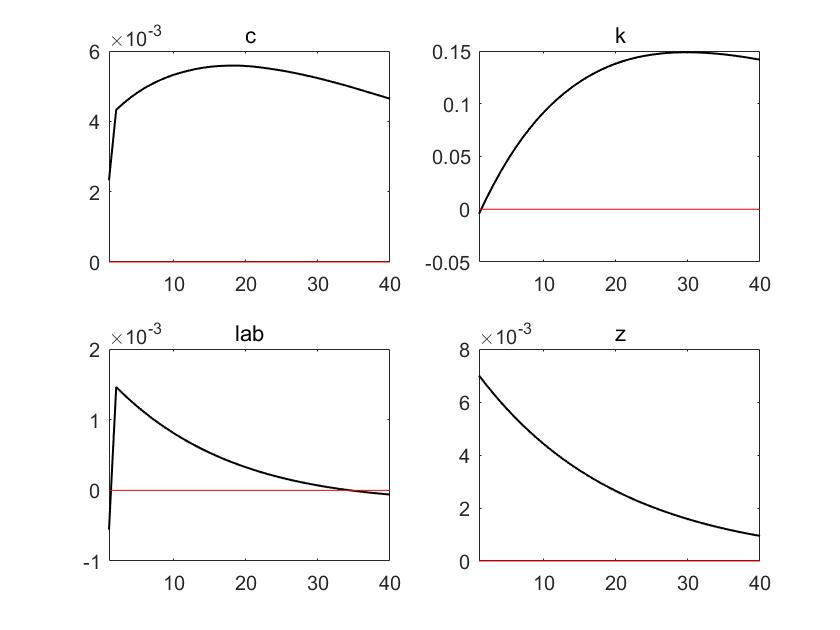
\includegraphics[width=0.6\linewidth]{fig1.jpg}
            \caption{Impulse response function to a technology shock}\label{1}
\end{figure}



\subsection{Estimation}

The simulated data series for consumption are used to estimate some unknown parameters of the model. Suppose we would like to estimate the preference parameters $\theta$ and $\tau$, and the stochastic process for productivity, summarized by two parameters $\rho$ and $\sigma$. The following code instructs Dynare to conduct the estimation.
\\
\textcolor{blue}{
var c k lab z;\\
varexo e;\\
\\
parameters bet del alp rho the tau s;\\
\\
bet     = 0.987;\\
the     = 0.357;\\
del     = 0.012;\\
alp     = 0.4;\\
tau     = 2;\\
rho     = 0.95;\\
s       = 0.007;\\
\\
model;\\
    (c\textasciicircum the*(1-lab)\textasciicircum(1-the))\textasciicircum(1-tau)/c=bet*((c(+1)\textasciicircum the*(1-lab(+1))\textasciicircum(1-the))\textasciicircum(1-tau)/c(+1))*(1+alp*exp(z(+1))*k\textasciicircum(alp-1)*lab(+1)\textasciicircum(1-alp)-del);\\
    c=the/(1-the)*(1-alp)*exp(z)*k(-1)\textasciicircum alp*lab\textasciicircum (-alp)*(1-lab);\\
    k=exp(z)*k(-1)\textasciicircum alp*lab\textasciicircum (1-alp)-c+(1-del)*k(-1);\\
    z=rho*z(-1)+s*e;\\
end;\\
\\
initval;\\
k   = 1;\\
c   = 1;\\
lab = 0.3;\\
z   = 0;\\
e   = 0;\\
end;\\
\\
shocks;\\
var e;\\
stderr 1;\\
end;\\
\\
estimated$\_$params;\\
stderr e, inv$\_$gamma$\_$pdf, 0.95,30;\\
rho, beta$\_$pdf,0.93,0.02;\\
the, normal$\_$pdf,0.3,0.05;\\
tau, normal$\_$pdf,2.1,0.3;\\
end;\\
\\
varobs c;\\
\\
estimation(datafile=simuldata,mode$\_$compute=6,mh$\_$replic=1000,mh$\_$jscale=0.9,nodiagnostic);}\\
\\

The priors used in estimation are as in Table 3. Table 4 is one of the outputs of Dynare which presents summary statistics of posterior distribution.

\begin{table}[h]
\centering\caption{Priors}\label{3}
\begin{tabular}{lccc}
  \hline
  Parameter&Distribution&Mean&Std.Dev.\\
  \hline
  $\rho$&Beta&0.93&0.02\\
  $\theta$&Normal&0.3&0.05\\
  $\tau$&Normal&2.1&0.3\\
  $\sigma$&Inv.Gamma&0.95&30\\
  \hline
  \end{tabular}
\end{table}

\begin{table}[h]
\centering\caption{Posteriors}\label{4}
\begin{tabular}{lcccccc}
  \hline
  Parameter&prior mean&post.mean&conf.&interval&prior dist.&prior Std.\\
  \hline
  $\rho$&0.9300&0.7451&0.7383&0.7530&beta&0.0200\\
  $\theta$&0.300&0.3542&0.3500&0.3582&norm&0.0500\\
  $\tau$&2.100&0.7613&0.7542&0.7689&norm&0.3000\\
  $\sigma$&0.9500&4.4338&4.3725&4.5074&invg&30.00\\
  \hline
  \end{tabular}
\end{table}


\begin{figure}[htbp!]
		\centering
			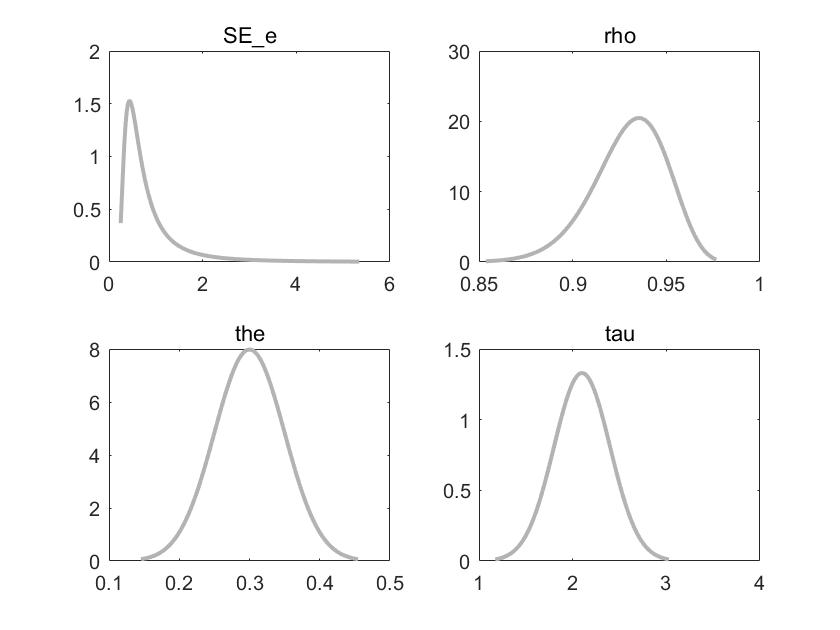
\includegraphics[width=0.7\linewidth]{fig2.jpg}
            \caption{Priors}\label{2}
\end{figure}

\begin{figure}[htbp!]
		\centering
			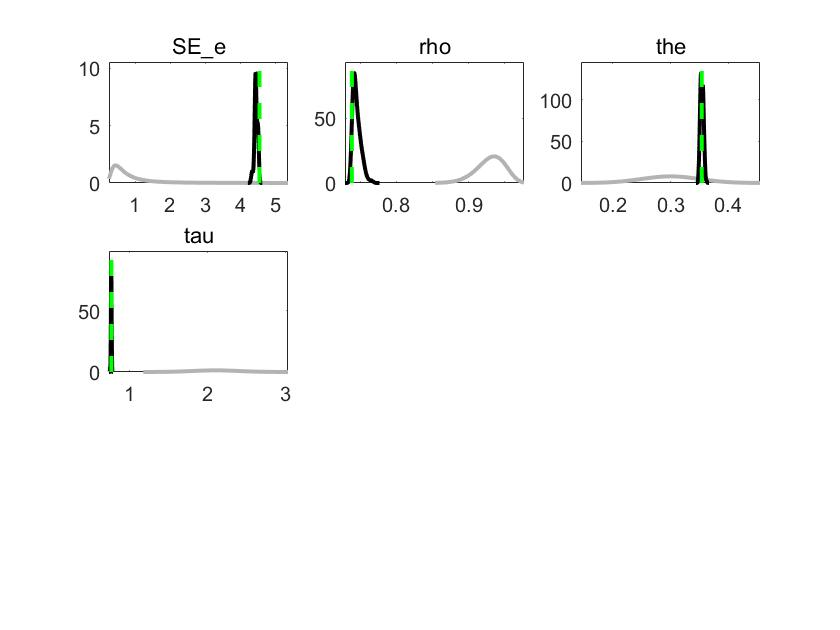
\includegraphics[width=0.8\linewidth]{fig3.jpg}
            \caption{Posteriors}\label{3}
\end{figure}


\section{International Business Cycle Model}

We study a simplified version of the two-country production model in Kim and Kim (2003).

\subsection{The model}

Two countries are identical ex-ante and markets are complete. A solution to a Pareto planner’s problem is characterized by the following equations

$$C_{1,t}=C_{2,t}$$
$$C_{1,t}^{-\gamma}=\beta E_tC_{1,t}^{-\gamma}(\alpha A_{1,t+1}K_{1,t+1}^{\alpha-1}+1-\delta$$
$$C_{2,t}^{-\gamma}=\beta E_tC_{2,t}^{-\gamma}(\alpha A_{2,t+1}K_{2,t+1}^{\alpha-1}+1-\delta$$
$$A_{1,t}K_{1,t}^{\alpha}+A_{2,t}K_{2,t}^{\alpha}=C_{1,t}+C_{2,t}+K_{1,t-1}-(1-\delta)K_{1,t}+K_{2,t-1}-(1-\delta)K_{2,t}$$
$$lnA_{1,t+1}=\rho lnA_{1,t}+\epsilon_{1,t+1}$$
$$lnA_{2,t+1}=\rho lnA_{2,t}+\epsilon_{2,t+1}$$

The first three equalities are the first-order conditions with regard to the consumption ($C_{i,t}$), and the fourth one is the world resource constraint. The last two describe the law of motion for the technological shock ($A_{i,t}$). $K_{i,t}$ denotes the capital stock of country i at time t.

\subsection{Calibration and approximation}
\subsubsection{Calibration}

The following parameter values are used.

\begin{table}[h]
\centering\caption{parameter calibration}\label{5}
\begin{tabular}{cc}
  \hline
  Parameter&Calibration\\
  \hline
  $\beta$&0.98\\
  $\delta$&0.05\\
  $\alpha$&0.4\\
  $\rho$&0.85\\
  $\sigma_{\epsilon_1}$&0.08\\
  $\sigma_{\epsilon_2}$&0.08\\
  \hline
  \end{tabular}
\end{table}

Dynare computes the policy function as a second-order approximation around the (log) steady-state. The .mod Dynare file of the system is as follows.\\
\\
\textcolor{blue}{
var c1 c2 k1 k2 a1 a2;\\
varexo e1 e2;\\
\\
parameters gamma delta alpha beta rho;\\
\\
gamma=2;\\
delta=.05;\\
alpha=.4;\\
beta=.98;\\
rho=.85;\\
\\
model;\\
c1=c2;\\
exp(c1)\textasciicircum(-gamma) =beta*exp(c1(+1))\textasciicircum(-gamma)*(alpha*exp(a1(+1))*exp(k1)\textasciicircum(alpha-1)+1-delta);\\
exp(c2)\textasciicircum(-gamma) =beta*exp(c2(+1))\textasciicircum(-gamma)*(alpha*exp(a2(+1))*exp(k2)\textasciicircum(alpha-1)+1-delta);\\
exp(c1)+exp(c2)+exp(k1)-exp(k1(-1))*(1-delta)+exp(k2)-exp(k2(-1))*(1-delta)= exp(a1)*exp(k1(-1))\textasciicircum alpha+exp(a2)*exp(k2(-1))\textasciicircum alpha;\\
a1=rho*a1(-1)+e1;\\
a2=rho*a2(-1)+e2;\\
end;\\
\\
initval;\\
k1=2.8;\\
k2=2.8;\\
c1=.8;\\
c2=.8;\\
a1=0;\\
a2=0;\\
e1=0;\\
e2=0;\\
end;\\
\\
shocks;\\
var e1;\\
stderr .08;\\
var e2;\\
stderr .08;\\
end;\\
\\
steady;\\
\\
stoch\_simul(periods=1000);}\\

The output is given as a matrix of coefficients for the policy function. From this matrix, for example, one can construct the optimal consumption rule for Country 1:

\begin{equation}\nonumber
\begin{split}
\hat{c}_{1,t}=&0.004+0.243(\hat{k}_{1,t-1}+\hat{k}_{2,t-1})+0.119(\hat{a}_{1,t-1}+\hat{a}_{2,t-1})\\
             &+0.140(\hat{e}_{1,t}+\hat{e}_{2,t})+0.062(\hat{k}_{1,t-1}^2+\hat{k}_{2,t-1}^2)\\
             &-0.110\hat{k}_{1,t-1}\hat{k}_{2,t-1}-0.013(\hat{k}_{1,t-1}\hat{a}_{1,t-1}+\hat{k}_{2,t-1}\hat{a}_{2,t-1})\\
            &- 0.027(\hat{k}_{2,t-1}\hat{a}_{1,t-1}+\hat{k}_{1,t-1}\hat{a}_{2,t-1})+0.032(\hat{a}_{1,t-1}^2+\hat{a}_{2,t-1}^2)\\
             &-0.029\hat{a}_{1,t-1}\hat{a}_{2,t-1}+0.044(\hat{e}_{1,t}^2+\hat{e}_{2,t}^2)-0.040\hat{e}_{1,t}\hat{e}_{2,t}\\
            & -0.015(\hat{k}_{1,t-1}\hat{e}_{1,t}+\hat{k}_{2,t-1}\hat{e}_{2,t})+0.075(\hat{a}_{1,t-1}\hat{e}_{1,t}+\hat{a}_{2,t-1}\hat{e}_{2,t})\\
            &-0.34(\hat{a}_{1,t-1}\hat{e}_{2,t}+\hat{a}_{2,t-1}\hat{e}_{1,t})
\end{split}
\end{equation}

where $\hat{c}$ denotes the deviation of $lnC$ from its log steady-state. Note that Dynare breaks $\hat{a}_{i,t}$ into $\hat{a}_{i,t-1}$ and $\epsilon_{i,t}$, so the output from Dynare looks unnecessarily messy.

Dynare also produces the associated impulse response functions of the system. Figure 4 illustrate the response of the system to a one-standard-deviation shock to $\epsilon_1$.

\begin{figure}[htbp!]
		\centering
			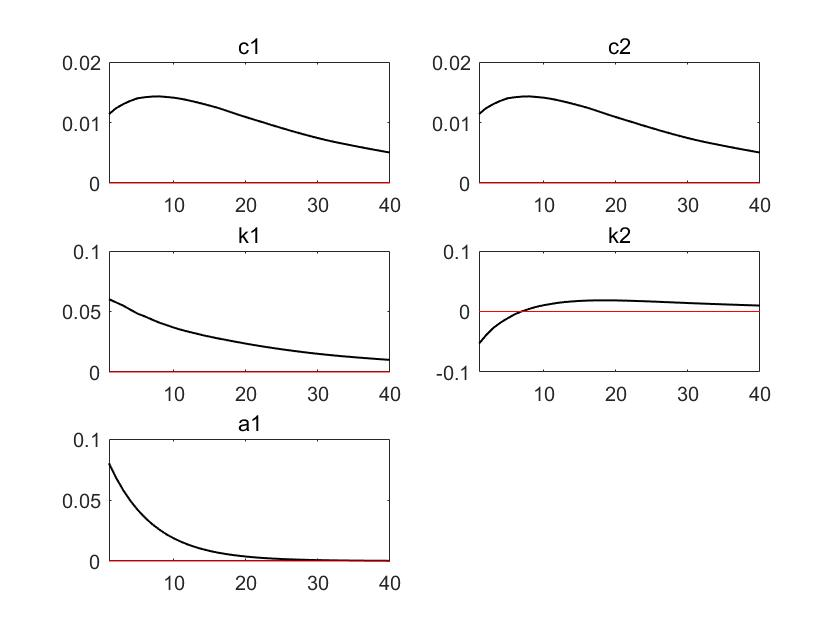
\includegraphics[width=0.8\linewidth]{fig4.jpg}
            \caption{Impulse response function($\epsilon_1$)}\label{4}
\end{figure}

The last line of the code generates sample paths of the variables governed by the approximated policy functions.

\subsection{Estimation}

Now assume that we do not know the true parameter values. We can estimate the unknown parameters from the saved data, using the Bayesian econometrics function of Dynare.

We will estimate 4 parameters $\rho, \alpha, \sigma_{\epsilon_1}$ and $\sigma_{\epsilon_2}$ . Hence, we have to specify the prior distribution of each parameter. In this exercise, $\rho, \alpha$ are given a normal prior, while the priors of $ \sigma_{\epsilon_1}$ and $\sigma_{\epsilon_2}$ are inverse gamma distributions. The Dynare code is as follows.\\
\\
\textcolor{blue}{
var c1 c2 k1 k2 a1 a2;\\
varexo e1 e2;\\
\\
parameters gamma delta alpha beta rho;\\
\\
gamma=2;\\
delta=.05;\\
alpha=.4;\\
beta=.98;\\
rho=.85;\\
\\
model;\\
c1=c2;
exp(c1)\^(-gamma)=beta*exp(c1(+1))\^(-gamma)*(alpha*exp(a1(+1))*exp(k1)\^(alpha-1)+1-delta);\\
exp(c2)\^(-gamma)=beta*exp(c2(+1))\^(-gamma)*(alpha*exp(a2(+1))*exp(k2)\^(alpha-1)+1-delta);\\
exp(c1)+exp(c2)+exp(k1)-exp(k1(-1))*(1-delta)+exp(k2)-exp(k2(-1))*(1-delta)=exp(a1)*exp(k1(-1))\^alpha+exp(a2)*exp(k2(-1))\^alpha;\\
a1=rho*a1(-1)+e1;\\
a2=rho*a2(-1)+e2;\\
end;\\
\\
initval;\\
k1=2.8;\\
k2=2.8;\\
c1=.8;\\
c2=.8;\\
a1=0;\\
a2=0;\\
e1=0;\\
e2=0;\\
end;\\
\\
shocks;\\
var e1;\\
stderr .08;\\
var e2;\\
stderr .08;\\
end;\\
\\
steady;\\
\\
estimated\_params;\\
rho, normal\_pdf, .84,.05;\\
alpha, normal\_pdf, .38, .03;\\
stderr e1, inv\_gamma\_pdf, .078, inf;\\
stderr e2,inv\_gamma\_pdf,.082, inf;\\
end;\\
\\
varobs c1 k2;\\
\\
estimation(datafile=simuldata\_international,mode\_compute=6,mh\_replic=1000,mh\_jscale=.5);}\\

Given that there are two exogenous shock variables, we use two observables $lnC_1$ and $lnK_2$. The result of the estimation is summarized in Figure 5, where the posterior distribution (in the darker line) of each parameter is contrasted against the given prior distribution. The result can be compared to the true parameter values in Table 5.

\begin{figure}[htbp!]
		\centering
			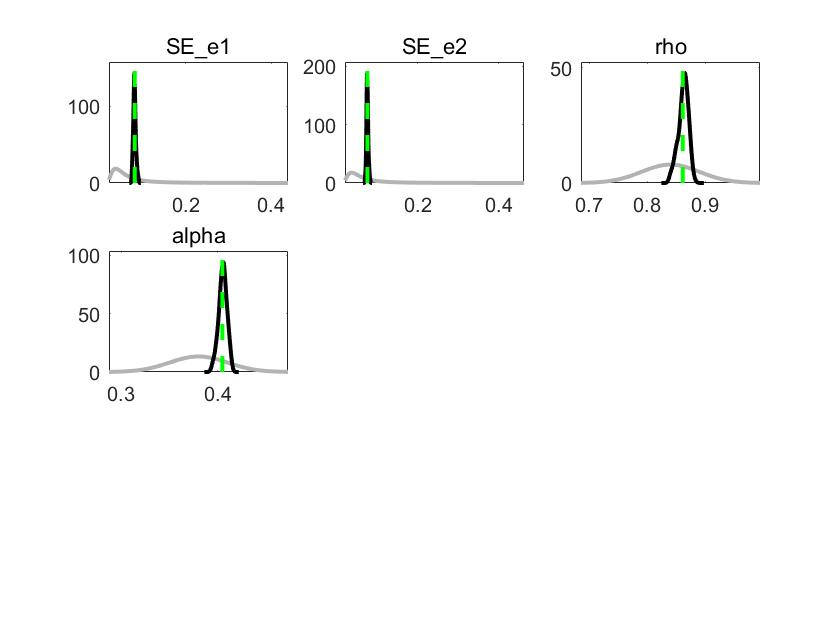
\includegraphics[width=0.8\linewidth]{fig5.jpg}
            \caption{Prior v. Posterior Distribution}\label{5}
\end{figure}

\section{Fiscal policies in the growth model}

This section describes a suite of Dynare programs that replicate the transition experiments performed in chapter 11 of Ljungqvist and Sargent (2004).

\subsection{The model}

A deterministic growth model has inelastic labor supply, an exogenous stream of government expenditures, and several kinds of distorting taxes. All variables are as described in chapter 11 of Ljungqvist and Sargent (2004). A representative agent maximizes

$$\sum_{t=0}^{\infty}\beta^t\frac{c_t^{1-\gamma}}{1-\gamma},~\beta \in (0,1)$$

Feasible allocations satisfy

$$g_t+c_t+k_{t+1}\le A_tK_t^{\alpha}+(1-delta)k_t$$

The household budget constraint is

$$\sum_{t=0}^{\infty}\{q_t(1+\tau_{c,t})+(1-\tau_{i,t})q_t[k_{t+1}-(1-\delta)k_t]\}\le \sum_{t=0}^{\infty}\{r_t(1-\tau_{k,t})k_t+w_t\}$$

and the government budget constraint is

$$\sum_{t=0}^{\infty}q_tg_t\le \sum_{t=0}^{\infty}\{\tau_{c,t}q_tc_t-\tau_{i,t}q_t[k_{t+1}-(1-\delta)k_t]+r_t\tau_{k,t}k_t+w_t\}$$

The following conditions characterize an equilibrium:

\begin{equation}\label{7}
   c_t=A_tk_t^{\alpha}+(1-\delta)k_t-k_{t+1}-g_t
\end{equation}
\begin{equation}\label{8}
   q_t=\beta^t\frac{c_t^{1-\gamma}}{1+\tau_{c,t}}
\end{equation}
\begin{equation}\label{9}
   \frac{r_t}{q_t}=A_t\alpha k_t^(\alpha-1)
\end{equation}
\begin{equation}\label{10}
    \frac{w_t}{q_t}=A_tk_t^(\alpha)-k_tA_t\alpha k_t^(\alpha-1)
\end{equation}
\begin{equation}\label{11}
    R_{t+1}=\frac{1+\tau_{c,t}}{1+\tau_{c,t+1}}[\frac{1+\tau_{i,t+1}}{1+\tau_{i,t}}(1-\delta)+\frac{1+\tau_{k,t+1}}{1+\tau_{k,t}}A_th=k_{t+1}^{\alpha-1}]
\end{equation}
\begin{equation}\label{12}
    \frac{s_t}{q_t}=(1-\tau_{k,t})A_t\alpha k_t^{\alpha-1}+(1-\delta)
\end{equation}
\begin{equation}\label{13}
    c_t^{-\gamma}=\beta c_{t+1}^{-\gamma}R_{t+1}
\end{equation}

Because the other endogenous variables can be expressed as functions of $k_t$ and $c_t$, in the programs below we use only a subset of the equilibrium conditions to compute equilibrium paths.

\subsection{Parameter values}

We set the parameters and the baseline values of the exogenous variables at values set in chapter 11 of Ljungqvist and Sargent (2004), as described in the following table 6 are taken from RMT2.

\begin{table}[h]
\centering\caption{parameter calibration}\label{6}
\begin{tabular}{cc}
  \hline
  Parameter&Calibration\\
  \hline
  $\beta$&0.95\\
  $\delta$&0.2\\
  $A$&1\\
  $\alpha$&0.33\\
  $\gamma$&2\\
  $g$&0.2\\
  $\tau_c$&0\\
  $\tau_i$&0\\
  $\tau_k$&0\\
  \hline
  \end{tabular}
\end{table}

\subsection{Transition experiments}
\subsubsection{A permanent increase in g}

The Dynare code below reproduces Figure 6. which looks at the impact of a permanent increase of 0.2 in g at t=10.\\
\\
\textcolor{blue}{
\% This program replicates figure 11.3.1 from chapter 11 of RMT2 by\\
\% Ljungqvist and Sargent.\\
\% y\_ records the simulated endogenous variables in alphabetical order\\
\% ys0\_ records the initial steady state\\
\% ys\_ records the terminal steady state\\
\% We check that these line up at the end points\\
\% Note: y\_ has ys0\_ in the first column, ys\_ in the last column, which explains\\
\% why it has 102 elements.\\
\% The sample of size 100 is in between.\\
\% Warning: All endogenous variables dated time t are treated as jump variables\\
\% in Dynare. So k in the program corresponds to k\_{t+1}\\
\% and the same timing holds for the taxes.\\
\% Declares the endogenous variables;\\
\\
var c k;\\
\\
\% declares the exogenous variables\\
\% investment tax credit, consumption tax, capital tax, government spending\\
\\
varexo taui tauc tauk g;\\
\\
parameters bet gam del alpha A;\\
\\
bet=.95; \% discount factor\\
gam=2; \% CRRA parameter\\
del=.2; \% depreciation rate\\
alpha=.33; \% capital’s share\\
A=1; \% productivity\\
\\
\% Alignment convention:\\
\% g tauc taui tauk are now columns of ex\_. Because of a bad design decision\\
\% the date of ex\_(1,:) doesn’t necessarily match the date in y\_.\\
\% Whether they match depends on the number of lag periods in endogenous versus\\
\% exogenous variables.\\
\% In this example they match because tauc(-1) and taui(-1) enter the model.\\
\% These decisions and the timing conventions mean that y\_(:,1) records the\\
\% initial steady state, while y\_(:,102) records the terminal steady state\\
\% values. For j > 2, y\_(:,j) records [c(j-1) .. k(j-1) .. G(j-1)] where k(j-1)\\
\% means end of period capital in period j-1, which equals k(j) in chapter 11\\
\% notation. Note that the jump in G occurs in y\_(;,11), which confirms this\\
\% timing. The jump occurs now in ex\_(11,1)\\
\\
model;\\
\% equation 11.3.8.a\\
k=A*k(-1)\^alpha+(1-del)*k(-1)-c-g;\\
\% equation 11.3.8e + 11.3.8.g\\
c\^(-gam)=bet*(c(+1)\^(-gam))*((1+tauc(-1))/(1+tauc))*((1-taui)*(1-del)/(1-taui(-1))+((1-tauk)/(1-taui(-1)))*alpha*A*k(-1)\^(alpha-1));\\
end;\\
\\
initval;\\
k=1.5;\\
c=0.6;\\
g = 0.2;\\
tauc = 0;\\
taui = 0;\\
tauk = 0;\\
end;\\
\\
steady; \% put this in if you want to start from the initial\\
\% steady state, comment it out to start from the indicated values\\
\\
endval; \% The following values determine the new steady state\\
\% after the shocks.\\
k=1.5;\\
c=0.4;\\
g =.4;\\
tauc =0;\\
taui =0;\\
tauk =0;\\
end;\\
\\
steady; \% We use steady again and the enval provided are initial\
\% guesses for Dynare to compute the ss.\\
\% The following lines produce a g sequence with a once and for all jump in g shocks\\
\% we use shocks to undo that for the first 9 periods and leave g at\\
\% it’s initial value of 0.2\\
\\
shocks;\\
var g;\\
periods 1:9;\\
values 0.2;\\
end;\\
\\
\% now solve the model\\
\\
simul(periods=100);\\
\\
\% Note: y\_ records the simulated endogenous variables in order of declaration\\
\% ys0\_ records the initial steady state\\
\% ys\_ records the terminal steady state\\
\% check that these line up at the end points\\
load('neoclassical\_fiscal\_results.mat', 'oo\_');\\
y\_=oo\_.endo\_simul;\\
ys0\_(:)=y\_(:,1);\\
ys\_(:)=y\_(:,102);\\
\\
\% Compute the initial steady state for consumption to later do the plots.\\
c0=y\_(1,1);\\
k0 = y\_(2,1);\\
\% g is in oo\_.exo\_simul(:,4) since it is stored in order of declaration\\
g0 = oo\_.exo\_simul(1,4);\\
\\
\% The following equation compute the other endogenous variables use in the plots below\\
\% Since they are function of capital and consumption, so we can compute them from the solved\\
\% model above.\\
\\
\%% These equations were taken from page 333 of RMT2\\
\\
rbig0=1/bet;\\
rbig=y\_(1,2:101).\^(-gam)./(bet*y\_(1,3:102).\^(-gam));\\
rq0=alpha*A*k0\^(alpha-1);\\
rq=alpha*A*y\_(2,1:100).\^(alpha-1);\\
wq0=A*k0\^alpha-k0*alpha*A*k0\^(alpha-1);\\
wq=A*y\_(2,1:100).\^alpha-y\_(2,1:100).*alpha*A.*y\_(2,1:100).\^(alpha-1);\\
sq0=(1-oo\_.exo\_simul(1,3))*A*alpha*k0\^(alpha-1)+(1-del);\\
sq=(1-oo\_.exo\_simul(1:100,3)')*A*alpha.*y\_(2,1:100).\^(alpha-1)+(1-del);\\
\\
\%Now we plot the responses of the endogenous variables to the shock.\\
\\
figure\\
subplot(2,3,1)\\
plot([k0*ones(100,1) y\_(2,1:100)' ]) \% note the timing: we lag capital to correct for syntax\\
title('k')\\
subplot(2,3,2)\\
plot([c0*ones(100,1)  y\_(1,2:101)' ])\\
title('c')\\
subplot(2,3,3)\\
plot([rbig0*ones(100,1) rbig' ])\\
title('R')\\
subplot(2,3,4)\\
plot([wq0*ones(100,1) wq' ])\\
title('w/q')\\
subplot(2,3,5)\\
plot([sq0*ones(100,1) sq' ])\\
title('s/q')\\
subplot(2,3,6)\\
plot([rq0*ones(100,1) rq' ])\\
title('r/q')}\\


The following figure 6 shows the path of the endogenous variables along the transition to the new steady state.

\begin{figure}[htbp!]
		\centering
			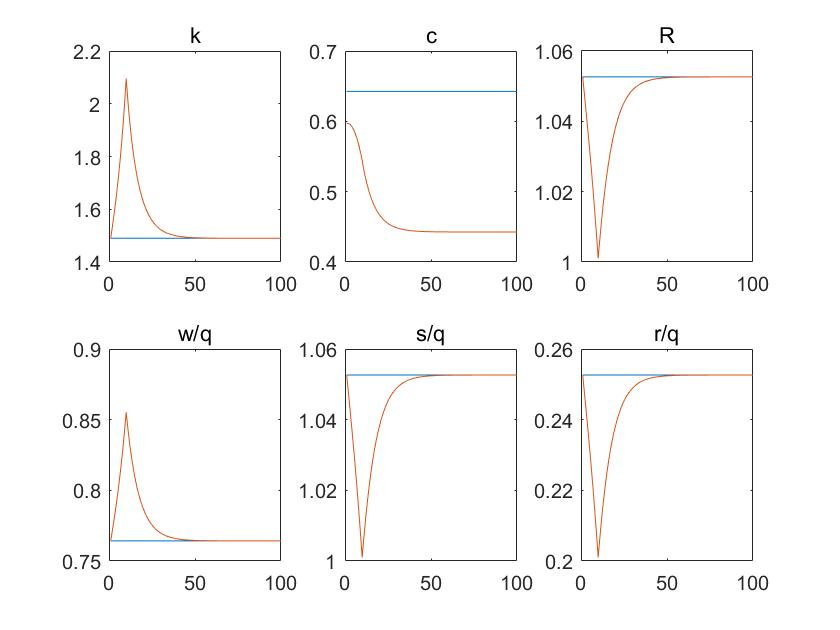
\includegraphics[width=0.8\linewidth]{fig6.jpg}
            \caption{A permanent increase of g}\label{6}
\end{figure}

\vspace{10cm}
Next we show the other transition experiments and only the parts of the code that need to be changed for each experiment.

\subsubsection{A permanent increase in $\tau_c$}

A permanent increase of $\tau_c$ at t=10 of 20 percent(Figure 7).\\
\\
\textcolor{blue}{
initval;\\
k=1.5;\\
c=0.6;\\
g = 0.2;\\
tauc = 0;\\
taui = 0;\\
tauk = 0;\\
end;\\
\\
steady;\\
\\
endval;\\
k=1.5;\\
c=0.6;\\
g = 0.2;\\
tauc =0.2;\\
taui =0;\\
tauk =0;\\
end;
\\
shocks;\\
var tauc;\\
periods 1:9;\\
values 0;\\
end;}\\

\begin{figure}[htbp!]
		\centering
			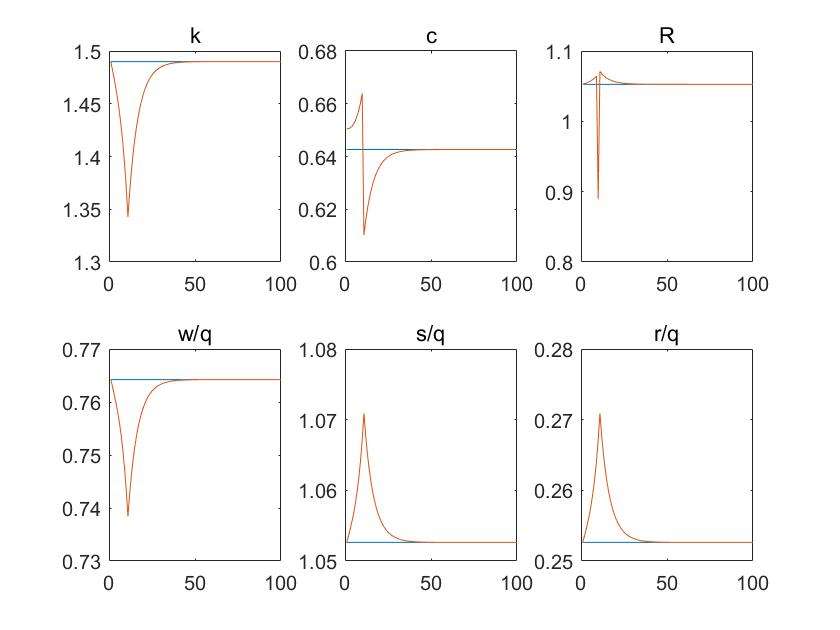
\includegraphics[width=0.8\linewidth]{fig7.jpg}
            \caption{A permanent increase of $\tau_c$}\label{6}
\end{figure}

\subsubsection{A permanent increase in $\tau_i$}

A permanent increase of $\tau_i$ at t=10 of 20 percent(Figure 8).\\
\\
\textcolor{blue}{
initval;\\
k=1.5;\\
c=0.6;\\
g = 0.2;\\
tauc = 0;\\
taui = 0;\\
tauk = 0;\\
end;\\
\\
steady;\\
\\
endval;\\
k=1.5;\\
c=0.6;\\
g =0.2;\\
tauc =0;\\
taui =0.20;\\
tauk =0;\\
end;\\
\\
steady;\\
\\
shocks;\\
var taui;\\
periods 1:9;\\
values 0;\\
end;}\\

\begin{figure}[htbp!]
		\centering
			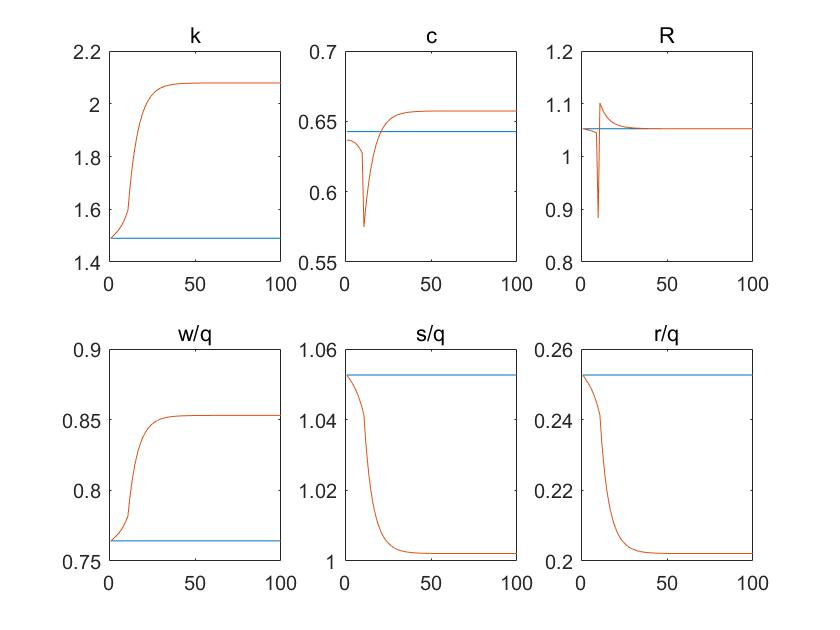
\includegraphics[width=0.8\linewidth]{fig8.jpg}
            \caption{A permanent increase of $\tau_i$}\label{8}
\end{figure}

\vspace{8cm}
~~
\subsubsection{A permanent increase in $\tau_k$}

A permanent increase of $\tau_k$ at t=10 of 20 percent(Figure 9).\\
\\
\textcolor{blue}{
initval;\\
k=1.5;\\
c=0.6;\\
g = 0.2;\\
tauc = 0;\\
taui = 0;\\
tauk = 0;\\
end;\\
\\
steady;\\
\\
endval;\\
k=1.5;\\
c=0.6;\\
g =0.2;\\
tauc =0;\\
taui =0;\\
tauk = 0.2;\\
end;\\
\\
steady;\\
\\
shocks;\\
var tauk;\\
periods 1:9;\\
values 0;\\
end;}\\

\begin{figure}[htbp!]
		\centering
			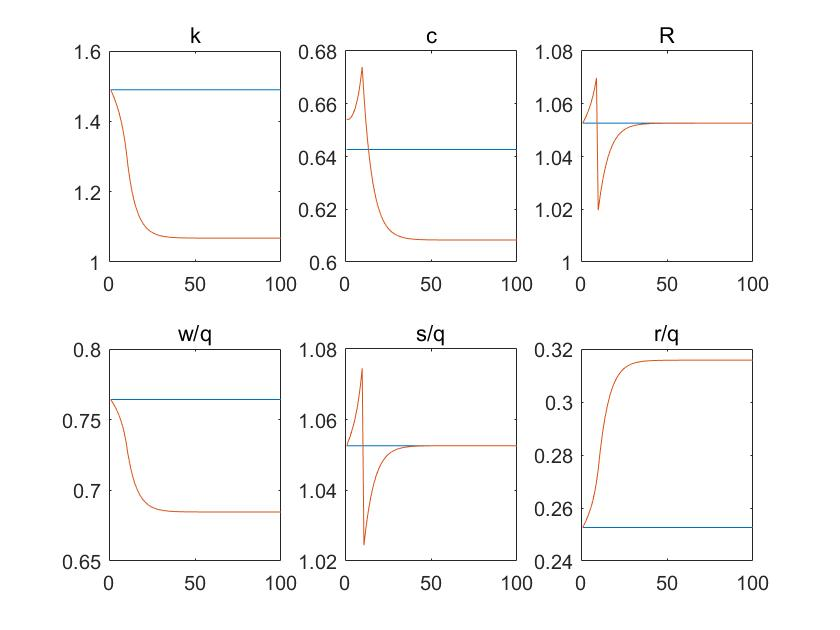
\includegraphics[width=0.8\linewidth]{fig9.jpg}
            \caption{A permanent increase of $\tau_k$}\label{9}
\end{figure}



\subsubsection{One time increase in g}

A one time pulse of g at t=10 of 0.2. (Figure 10)\\
\\
\textcolor{blue}{
initval;\\
k=1.5;\\
c=0.6;\\
g = 0.2;\\
tauc = 0;\\
taui = 0;\\
tauk = 0;\\
end;\\
\\
steady;\\
\\
endval;\\
k=1.5;\\
c=0.6;\\
g = 0.2;\\
tauc =0;\\
taui =0;\\
tauk =0;\\
end;\\
\\
steady;\\
\\
shocks;\\
var g;\\
periods 10;\\
values 0.4;\\
end;}\\

\begin{figure}[htbp!]
		\centering
			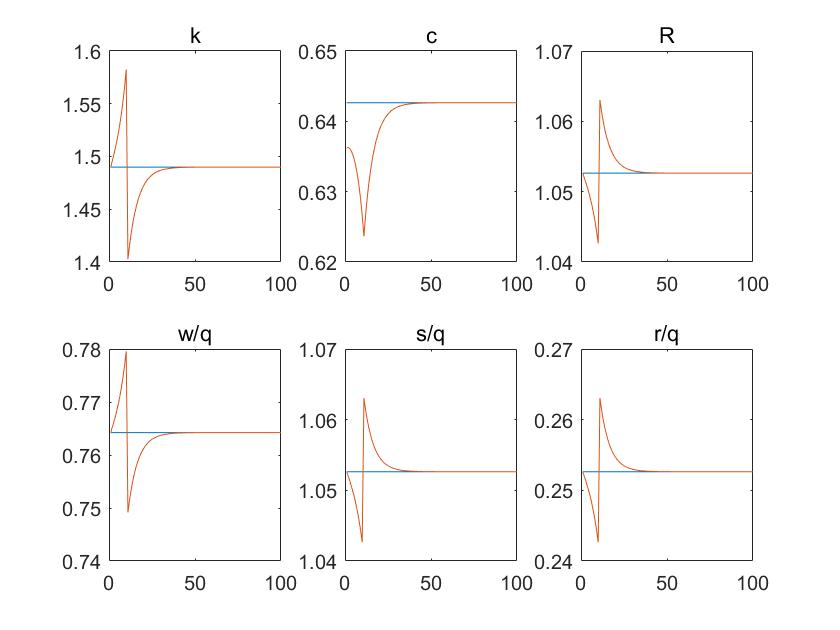
\includegraphics[width=0.8\linewidth]{fig10.jpg}
            \caption{One time increase of g}\label{10}
\end{figure}

\vspace{8cm}

\subsubsection{One time increase in $\tau_i$}

A one time pulse of $\tau_i$ at t=10 of 20 percent. (Figure 11)\\
\\
\textcolor{blue}{
initval;\\
k=1.5;\\
c=0.6;\\
g = 0.2;\\
tauc = 0;\\
taui = 0;\\
tauk = 0;\\
end;\\
\\
steady;\\
\\
endval;\\
k=1.5;\\
c=0.6;\\
g =0.2;\\
tauc =0;\\
taui =0;\\
tauk =0;\\
end;\\
\\
steady;\\
\\
shocks;\\
var taui;\\
periods 10;\\
values 0.2;\\
end;}\\

\begin{figure}[htbp!]
		\centering
			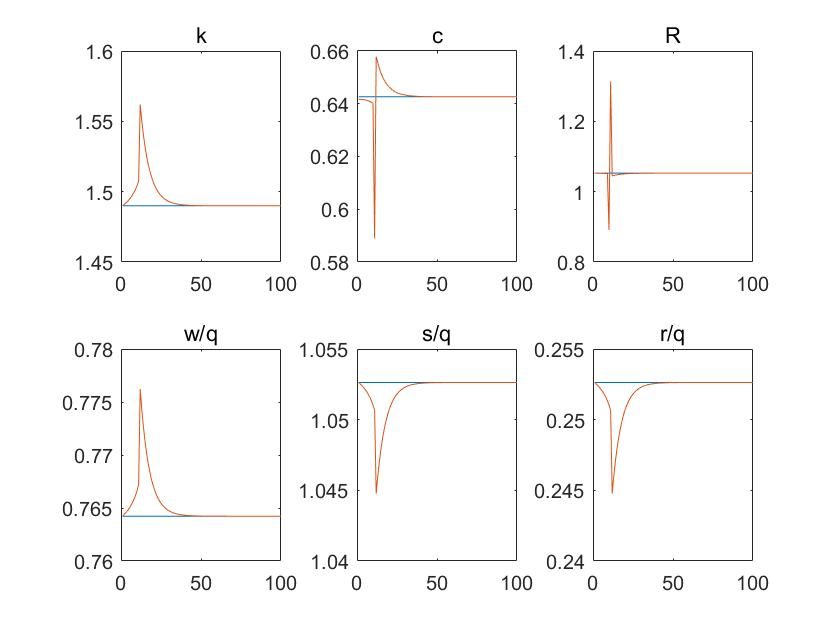
\includegraphics[width=0.8\linewidth]{fig11.jpg}
            \caption{One time increase of g}\label{11}
\end{figure}

\section{Fiscal policies in the growth model}

This section describes a suite of Dynare programs that replicate the transition experiments performed in chapter 11 of Ljungqvist and Sargent (2004).

\subsection{The model with inelastic labor supply}
A deterministic growth model has inelastic labor supply, an exogenous stream of government expenditures, and several kinds of distorting taxes. All variables are as described in chapter 11 of Ljungqvist and Sargent (2004). A representative agent maximizes

$$\sum_{t=0}^{\infty}\beta^t\frac{c_t^{1-\gamma}}{1-\gamma},~\beta \in (0,1)$$

Feasible allocations satisfy

$$g_t+c_t+k_{t+1}\le A_tK_t^{\alpha}+(1-delta)k_t$$

The household budget constraint is

$$\sum_{t=0}^{\infty}\{q_tc_t(1+\tau_{c,t})+q_t[k_{t+1}-(1-\delta)k_t]\}\le \sum_{t=0}^{\infty}q_t\{\eta_t(1-\tau_{k,t})k_t+w_t\}$$

and the government budget constraint is

$$\sum_{t=0}^{\infty}q_tg_t\le \sum_{t=0}^{\infty}q_t\{\tau_{c,t}c_t+\eta_t\tau_{k,t}k_t\}$$

The following conditions characterize an equilibrium:

\begin{equation}\label{14}
   c_t=A_tk_t^{\alpha}+(1-\delta)k_t-k_{t+1}-g_t
\end{equation}
\begin{equation}\label{15}
   q_t=\beta^t\frac{c_t^{-\gamma}}{1+\tau_{c,t}}
\end{equation}
\begin{equation}\label{16}
   \eta_t=A_t\alpha k_t^(\alpha-1)
\end{equation}
\begin{equation}\label{17}
    w_t=A_tk_t^(\alpha)-k_tA_t\alpha k_t^(\alpha-1)
\end{equation}
\begin{equation}\label{18}
    \hat{R}_{t+1}=\frac{1+\tau_{c,t}}{1+\tau_{c,t+1}}[(1-\delta)+(1-\tau_{k,t+1})A_t\alpha k_{t+1}^{\alpha-1}]
\end{equation}
\begin{equation}\label{19}
    c_t^{-\gamma}=\beta c_{t+1}^{-\gamma}\hat{R}_{t+1}
\end{equation}

Because the other endogenous variables can be expressed as functions of $k_t$ and $c_t$, in the programs below we use only a subset of the equilibrium conditions to compute equilibrium paths.

\subsection{Parameter values}

We set the parameters and the baseline values of the exogenous variables at values set in chapter 11 of Ljungqvist and Sargent (2004), as described in the following table 6 are taken from RMT2.

\begin{table}[h]
\centering\caption{parameter calibration}\label{7}
\begin{tabular}{cc}
  \hline
  Parameter&Calibration\\
  \hline
  $\beta$&0.95\\
  $\delta$&0.2\\
  $A$&1\\
  $\alpha$&0.33\\
  $\gamma$&2\\
  $g$&0.2\\
  $\tau_c$&0\\
  $\tau_k$&0\\
  \hline
  \end{tabular}
\end{table}

\subsection{Transition experiments}
\subsubsection{Foreseen once-and-for-all increase in g}

The Dynare code below reproduces Figure 12. which looks at the impact of a foreseen once-for-and-all increase of 0.2 in g at t = 10.\\
\\

\%-----------------------------------------------------------------------------------------------\\
\% Experiment  : Permenant increase in g at t=10\\
\% Note:Following the discussion in the text t = 0 is the first period of the new (simulated) path\\
\%-----------------------------------------------------------------------------------------------\\
\\
\% This program replicates figure 11.6.1 from chapter 11 of RMT3 by Ljungqvist and Sargent\\
\\
\% Dynare records the endogenous variables with the following convention.\\
\%Say N is the number of simulations(sample)\\
\%Index 1 : Initial values (steady sate)\\
\%Index 2 to N+1 : N simulated values\\
\%Index N+2 : Terminal Value (Steady State)\\
\% Warning:  we align c, k, and the taxes to exploit the dynare syntax.\\
\%In Dynare the timing of the variable reflects the date when the variable is decided.\\
\%For instance the capital stock for time 't' is decided in time 't-1'(end of period).\\
\%So a statement like k(t+1) = i(t) + (1-del)*k(t) would translate to\\
\% k(t) = i(t) +(1-del)*k(t-1) in the code.\\
\\
\%-----------------------------------------------------------------------------------------------\\
\% 1. Defining variables\\
\%-----------------------------------------------------------------------------------------------\\
\\
\% Declares the endogenous variables consumption ('c') capital stock (k);\\
var c k;\\
\\
\% declares the exogenous variables consumption tax ('tauc'),\\
\% capital tax('tauk'), government spending('g')\\
varexo tauc tauk g;\\
\\
parameters bet gam del alpha A;\\
\\
\%-----------------------------------------------------------------------------------------------\\
\% 2. Calibration and alignment convention\\
\%-----------------------------------------------------------------------------------------------\\
\\
bet=.95;  \% discount factor\\
gam=2;    \% CRRA parameter\\
del=.2;  \%  depreciation rate\\
alpha=.33; \%  capital's share\\
A=1;    \% productivity\\
\\
\% Alignment convention:\\
\% g tauc tauk are now columns of ex\_. Because of a bad design decision  the date of ex\_(1,:)\\
\% doesn't necessarily match the date in endogenous variables. Whether they match depends on\\
\% the number of lag periods in endogenous versus exogenous variables.\\
\\
\% These decisions and the timing conventions mean that\\
\% k(1) records the initial steady state, while k(102) records the terminal steady state values.\\
\% For j > 1, k(j) records the variables for j-1th simulation where the capital stock decision\\
\% taken in j-1th simulation i.e stock at the beginning of period j.\\
\% The variable ex\_ also follows a different timing convention i.e\\
\% ex\_(j,:) records the value of exogenous variables in the jth simulation.\\
\% The jump in the government policy is reflected in ex\_(11,1) for instance.\\
\\
\%-----------------------------------------------------------------------------------------------\\
\% 3. Model\\
\%-----------------------------------------------------------------------------------------------\\
\\
model;\\
\% equation 11.3.8.a\\
\\
k=A*k(-1)\^alpha+(1-del)*k(-1)-c-g;\\
\\
\% equation 11.3.8e + 11.3.8.g\\
c\^(-gam)= bet*(c(+1)\^(-gam))*((1+tauc)/(1+tauc(+1)))*((1-del) + (1-tauk(+1))*alpha*A*k\^(alpha-1));\\
\\
end;\\
\\
\%-----------------------------------------------------------------------------------------------\\
\% 4. Computation\\
\%-----------------------------------------------------------------------------------------------\\
\\
initval;\\
k=1.5;\\
c=0.6;\\
g = .2;\\
tauc = 0;\\
tauk = 0;\\
end;\\
\\
steady;\\
\% put this in if you want to start from the initial steady state,comment it out to start\\
\% from the indicated values\\
\\
\% The following values determine the new steady state after the shocks.\\
endval;\\
k=1.5;\\
c=0.6;\\
g =.4;\\
tauc =0;\\
tauk =0;\\
end;\\
\\
steady;\\
\% We use 'steady' again and the endval provided are initial guesses for dynare to compute the ss.\\
\\
\% The following lines produce a g sequence with a once and for all jump in g\\
\% we use 'shocks' to undo that for the first 10 periods (t=0 until t=9)and leave g at\\
\% it's initial value of 0\\
\% Note :  period j refers to the value in the jth simulation\\
\\
shocks;\\
var g;\\
periods 1:10;\\
values 0.2;\\
end;\\
\\
\% now solve the model\\
simul(periods=100);\\
\\
\% Compute the initial steady state for consumption to later do the plots.\\
load('neoclassical\_fiscal\_fig12\_results.mat', 'oo\_');\\
c0=oo\_.endo\_simul(1,1);\\
k0 =oo\_.endo\_simul(2,1);\\
\% g is in oo\_.exo\_simul(:,1) since it is stored in order of declaration\\
g0 = oo\_.exo\_simul(1,3)\\
\\
\%-----------------------------------------------------------------------------------------------\\
\% 5. Graphs and plots for other endogenous variables\\
\%-----------------------------------------------------------------------------------------------\\
\\
\% Let N be the periods to plot\\
N=40;\\
\\
\% The following equation compute the other endogenous variables use in the plots below\\
\% Since they are function of capital and consumption, so we can compute them from the solved\\
\% model above.\\
\% These equations were taken from page 371 of RMT3\\
rbig0=1/bet;\\
rbig=oo\_.endo\_simul(1,2:101).\^(-gam)./(bet*oo\_.endo\_simul(1,3:102).\^(-gam));\\
nq0=alpha*A*k0\^(alpha-1);\\
nq=alpha*A*oo\_.endo\_simul(2,1:100).\^(alpha-1);\\
wq0=A*k0\^alpha-k0*alpha*A*k0\^(alpha-1);\\
wq=A*oo\_.endo\_simul(2,1:100).\^alpha-oo\_.endo\_simul(2,1:100).*alpha*A.*oo\_.endo\_simul(2,1:100).\^(alpha-1);\\
\\
\% Now we plot the responses of the endogenous variables to the shock.\\
x=0:N-1;\\
figure(1)\\
\\
\% subplot for capital 'k'\\
subplot(2,3,1)\\
plot(x,[k0*ones(N,1)],'--k', x,oo\_.endo\_simul(2,1:N),'k','LineWidth',1.5)\\
\% note the timing: we lag capital to correct for syntax\\
title('k','Fontsize',12)\\
set(gca,'Fontsize',12)\\
\\
\% subplot for consumption 'c'\\
subplot(2,3,2)\\
plot(x,[c0*ones(N,1)],'--k', x,oo\_.endo\_simul(1,2:N+1),'k','LineWidth',1.5)\\
title('c','Fontsize',12)\\
set(gca,'Fontsize',12)\\
\\
\% subplot for cost of capital 'R\_bar'\\
subplot(2,3,3)\\
plot(x,[rbig0*ones(N,1)],'--k', x,rbig(1:N),'k','LineWidth',1.5)\\
title('$\verb|\|$overline{R}','interpreter', 'latex','Fontsize',12)\\
set(gca,'Fontsize',12)\\
\\
\% subplot for rental rate 'eta'\\
subplot(2,3,4)\\
plot(x,[nq0*ones(N,1)],'--k', x,nq(1:N),'k','LineWidth',1.5)\\
title('$\verb|\|$eta','Fontsize',12)\\
set(gca,'Fontsize',12)\\
\\
\% subplot for the experiment proposed\\
subplot(2,3,5)\\
plot([0:9],oo\_.exo\_simul(1:10,3),'k','LineWidth',1.5);\\
hold on;\\
plot([10:N-1],oo\_.exo\_simul(11:N,3),'k','LineWidth',1.5);\\
hold on;\\
plot(x,[g0*ones(N,1)],'--k','LineWidth',1.5)\\
title('g','Fontsize',12)\\
axis([0 N -.1 .5])\\
set(gca,'Fontsize',12)\\



The following figure shows the path of the endogenous variables along the transition to the new steady state.

\begin{figure}[htbp!]
		\centering
			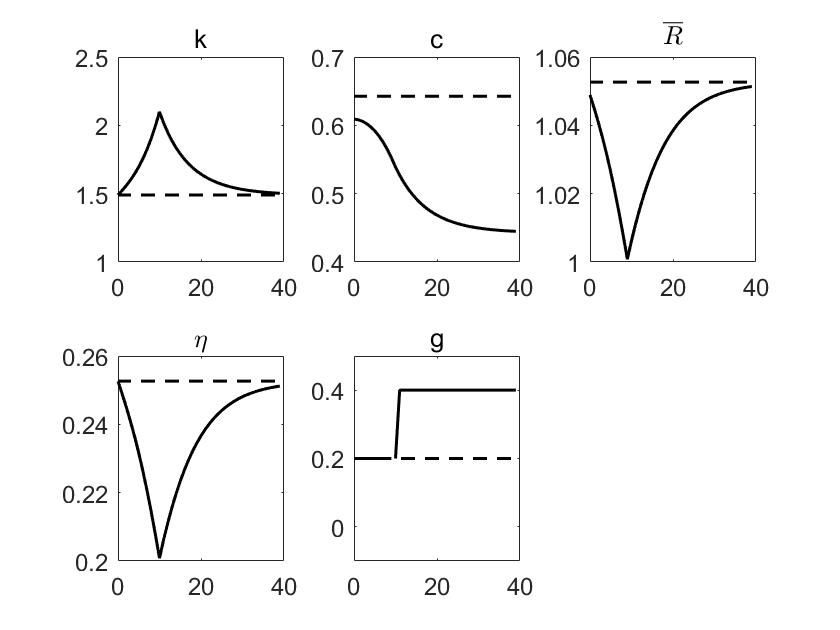
\includegraphics[width=0.8\linewidth]{fig12.jpg}
            \caption{Foreseen once-and-for-all increase in g at t = 10}\label{12}
\end{figure}

Next we show the other transition experiments and only the parts of the code that need to be changed for each experiment.

\subsubsection{Foreseen once-and-for-all increase in $\tau_c$}

A foreseen once-and-for-all increase in $\tau_c$ at t = 10 of 20 per cent.(Figure 13)\\
\\
\textcolor{blue}{
initval;\\
k=1.5;\\
c=0.6;\\
g = 0.2;\\
tauc = 0;\\
tauk = 0;\\
end;\\
\\
steady;\\
\\
endval;\\
k=1.5;\\
c=0.6;\\
g = 0.2;\\
tauc =0.2;\\
tauk =0;\\
end;\\
\\
steady;\\
\\
shocks;\\
var tauc;\\
periods 1:10;\\
values 0;\\
end;}\\

\begin{figure}[htbp!]
		\centering
			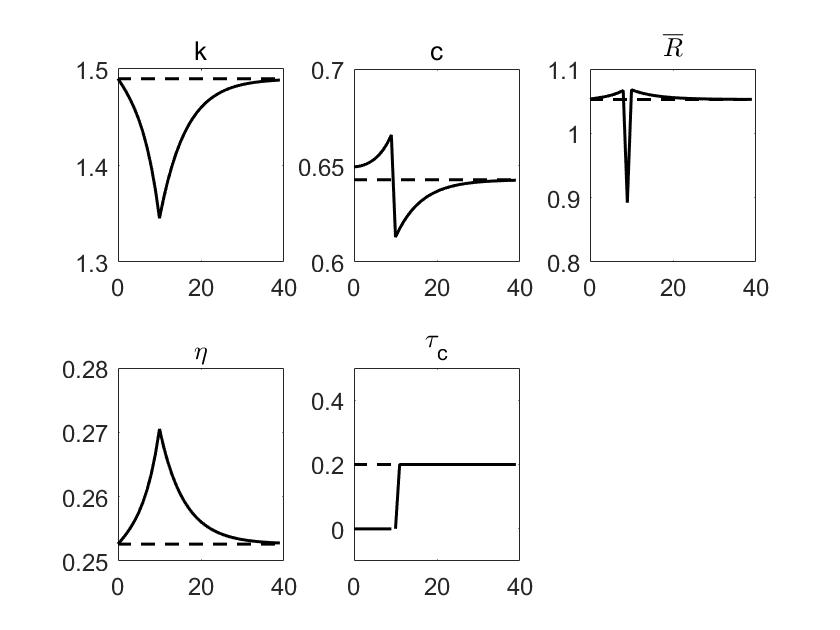
\includegraphics[width=0.8\linewidth]{fig13.jpg}
            \caption{Foreseen once-and-for-all increase in $\tau_c$ at t = 10}\label{13}
\end{figure}

\vspace{4cm}

\subsubsection{Foreseen once-and-for-all increase in $\tau_k$}

A foreseen once-and-for-all increase in $\tau_k$ at t = 10 of 20 per cent.(Figure 14)\\
\\
\textcolor{blue}{
initval;\\
k=1.5;\\
c=0.6;\\
g = 0.2;\\
tauc = 0;\\
tauk = 0;\\
end;\\
\\
steady;\\
\\
endval;\\
k=1.5;\\
c=0.6;\\
g =0.2;\\
tauc =0;\\
tauk = 0.2\\;
end;\\
\\
steady;\\
\\
shocks;\\
var tauk;\\
periods 1:10;\\
values 0;\\
end;}\\

\begin{figure}[htbp!]
		\centering
			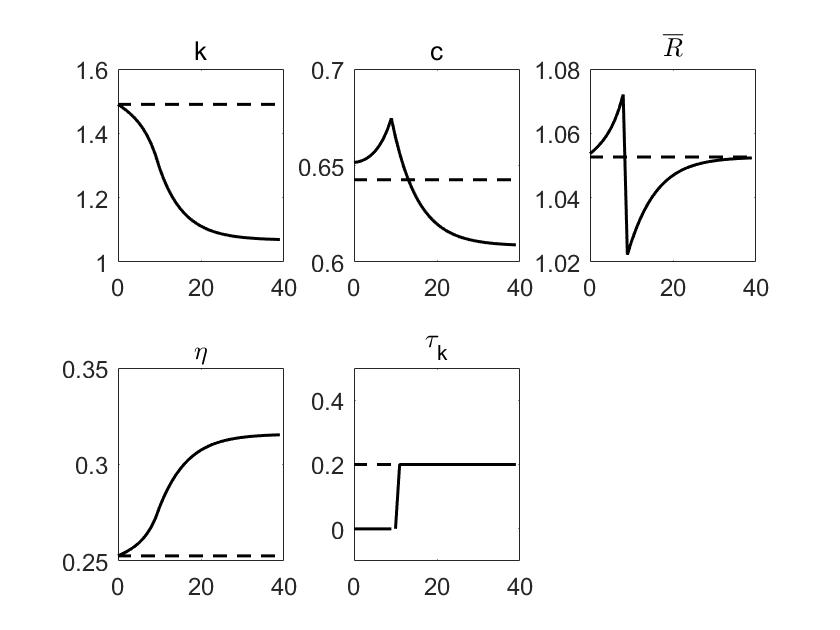
\includegraphics[width=0.8\linewidth]{fig14.jpg}
            \caption{Foreseen once-and-for-all increase in $\tau_k$ at t = 10}\label{14}
\end{figure}



\subsubsection{Foreseen one-time pulse increase in g}

A foreseen one-time pulse of g at t = 10 of 0.2. (Figure 15)\\
\\
\textcolor{blue}{
initval;\\
k=1.5;\\
c=0.6;\\
g = 0.2;\\
tauc = 0;\\
tauk = 0;\\
end;\\
\\
steady;\\
\\
endval;\\
k=1.5;\\
c=0.6;\\
g = 0.2;\\
tauc =0;\\
tauk =0;\\
end;\\
\\
steady;\\
shocks;\\
var g;\\
periods 11;\\
values 0.4;\\
end;}\\

\begin{figure}[htbp!]
		\centering
			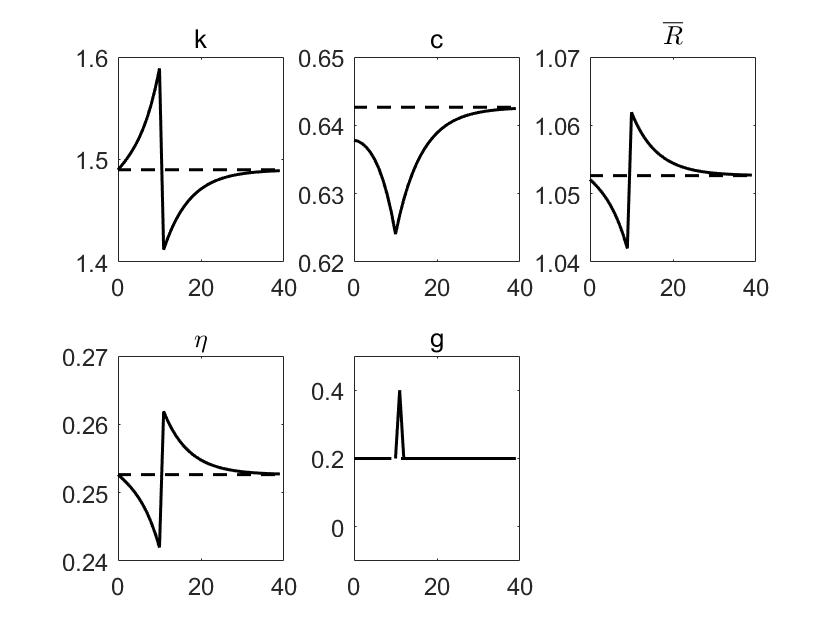
\includegraphics[width=0.8\linewidth]{fig15.jpg}
            \caption{Foreseen one-time pulse increase in g at t = 10}\label{15}
\end{figure}

\subsubsection{Foreseen once-and-for-all increase g at t = 10 for two economies}

Responses to a foreseen increase in g at t = 10 for two economies, the original economy with $\gamma=2$ and an otherwise identical economy with $\gamma=0.2$ (Figure 16).\\
\\
textcolor{blue}{
\% Compute the initial steady state for consumption to later do the plots.\\
c0=c(1);\\
k0= k(1);\\
\% g is in oo\_.exo\_simul(:,1) since it is stored in order of declaration\\
g0 = oo\_.exo\_simul(1,1);\\
\\
\%values for gamma = 2\\
kgamma(:,1)=k;\\
cgamma(:,1)=c;\\
rbig(:,1)=cgamma(2:101,1).\^(-gam)./(bet*cgamma(3:102,1).\^(-gam));\\
\\
\%values for gamma=.2\\
gam=.2;\\
simul(periods=100);\\
kgamma(:,2)=k;\\
cgamma(:,2)=c;\\
rbig(:,2)=cgamma(2:101,2).\^(-gam)./(bet*cgamma(3:102,2).\^(-gam));\\
\\
\%----------------------------------------------------------------\\
\% 5. Graphs and plots for other endogenous variables\\
\%----------------------------------------------------------------\\
\%Let N be the periods to plot\\
N=40;\\
\\
\% The following equation compute the other endogenous variables use in the plots below\\
\% Since they are function of capital and consumption, so we can compute them from the solved\\
\% model above.\\
\\
\% These equations were taken from page 371 of RMT3\\
rbig0=1/bet;\\
nq0=alpha*A*k0\^(alpha-1);\\
nq=alpha*A*kgamma(1:100,:).\^(alpha-1);\\
wq0=A*k0\^alpha-k0*alpha*A*k0\^(alpha-1);\\
wq=A*kgamma(1:100,:).\^alpha-kgamma(1:100,:).*alpha*A.*kgamma(1:100,:).\^(alpha-1);\\
\\
\%Now we plot the responses of the endogenous variables to the shock.\\
x=0:N-1;\\
figure(1)\\
\\
\% subplot for capital 'k'\\
subplot(2,3,1)\\
plot(x,[k0*ones(N,1)],'--k', x,kgamma(1:N,1),'k',x,kgamma(1:N,2),'-.k','LineWidth',1.5) \% note the timing: we lag capital to correct for syntax\\
title('k','Fontsize',12)\\
set(gca,'Fontsize',12)\\
\\
\% subplot for consumption 'c'\\
subplot(2,3,2)\\
plot(x,[c0*ones(N,1)],'--k', x,cgamma(2:N+1,1),'k',x,cgamma(2:N+1,2),'-.k','LineWidth',1.5)\\
title('c','Fontsize',12)\\
set(gca,'Fontsize',12)\\
\\
\% subplot for cost of capital 'R\_bar'\\
subplot(2,3,3)\\
plot(x,[rbig0*ones(N,1)],'--k', x,rbig(1:N,1),'k',x,rbig(1:N,2),'-.k','LineWidth',1.5)\\
title('$\verb|\|$overline{R}','interpreter', 'latex','Fontsize',12)\\
set(gca,'Fontsize',12)\\
\\
\% subplot for rental rate 'eta'\\
subplot(2,3,4)\\
plot(x,[nq0*ones(N,1)],'--k', x,nq(1:N,1),'k',x,nq(1:N,2),'-.k','LineWidth',1.5)\\
title('$\verb|\|$eta','Fontsize',12)\\
set(gca,'Fontsize',12)\\
legend('$\verb|\|$gamma=0.2','$\verb|\|$gamma=2')	\\
\\
\% subplot for the experiment proposed\\
subplot(2,3,5)\\
plot([0:9],oo\_.exo\_simul(1:10,3),'k','LineWidth',1.5);\\
hold on;\\
plot([10:N-1],oo\_.exo\_simul(11:N,3),'k','LineWidth',1.5);\\
hold on;\\
plot(x,[g0*ones(N,1)],'--k','LineWidth',1.5)\\
title('g','Fontsize',12)\\
axis([0 N -.1 .5])\\
set(gca,'Fontsize',12)}\\


\begin{figure}[htbp!]
		\centering
			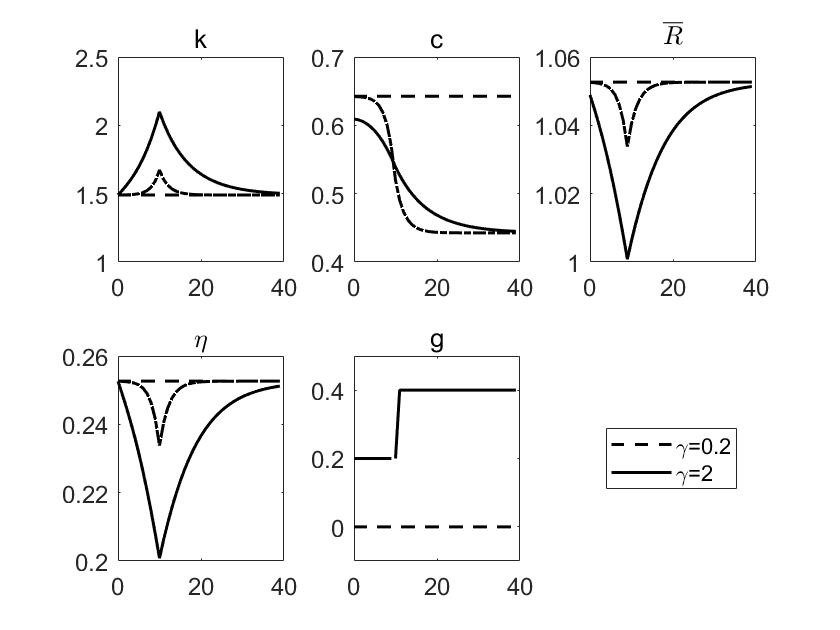
\includegraphics[width=0.8\linewidth]{fig16.jpg}
            \caption{Response to foreseen once-and-for-all increase in g at t = 10}\label{16}
\end{figure}

\subsubsection{Impact of an foreseen once-and-for-all increase in g on yield curves}

Impact of an foreseen once-and-for-all increase in g at t = 10 on yield curves. For this section we use some additional formulas

\begin{equation}\label{20}
    q_t=\frac{\beta^tc_t^{-\gamma}}{c_o^{-\gamma}}
\end{equation}
\begin{equation}\label{21}
    y_{i,t}=-\frac{1}{i}log(\frac{q_{t+i}}{q_t})
\end{equation}

\textcolor{blue}{
\%----------------------------------------------------------------\\
\% 5. Graphs and plots for other endogenous variables\\
\%----------------------------------------------------------------\\
\%Let N be the periods to plot\\
N=40;
\% The following equation compute the other endogenous variables use in the plots below\\
\% Since they are function of capital and consumption, so we can compute them from the solved\\
\% model above.\\
\\
\% These equations were taken from page 333 of RMT2\\
rbig0=1/bet;\\
rbig=c(2:101).\^(-gam)./(bet*c(3:102).\^(-gam));\\
nq0=alpha*A*k0\^(alpha-1);\\
nq=alpha*A*k(1:100).\^(alpha-1);\\
wq0=A*k0\^alpha-k0*alpha*A*k0\^(alpha-1);\\
wq=A*k(1:100).\^alpha-k(1:100).*alpha*A.*k(1:100).\^(alpha-1);\\
\\
\% computing the price system : q and steady state price system qs(t)=beta\^t\\
\%q(2) is normalized to 1\\
\%qs(1) is normalized to 1\\
for n=1:102\\
q(n)=bet\^n*c(n).\^(-gam)/(bet\^2*c(2)\^(-gam));\\
qs(n)=bet\^n*c(1).\^(-gam)/(bet*c(1)\^(-gam));\\
end\\
\\
\% computing the short term interest rates\\
\\
rsmall=-log(q(3:102)./q(2:101));\\
rsmall0=rbig0-1;\\
\\
\% computing the term structure for n=1 to 40 for all periods\\
\\
for t=1:62\\
for i=1:40\\
y(i,t)=log(q(i+t)/q(t))/-i;\\
end\\
end\\
\\
\%Now we plot the yield curves and other responses of the endogenous variables to the shock.\\
\\
figure(1)\\
x=0:N-1;\\
\% subplot for consumption 'c'\\
subplot(2,3,1)\\
plot(x,c0*ones(N,1),'--k', x,c(2:N+1),'k','LineWidth',1.5)\\
title('c','Fontsize',12)\\
set(gca,'Fontsize',12)\\
\\
\% subplot for consumption 'q'\\
subplot(2,3,2)\\
plot(x,qs(1:N),'--k', x,q(2:N+1),'k','LineWidth',1.5)\\
title('q','Fontsize',12)\\
set(gca,'Fontsize',12)\\
\\
\% subplot for rate of interest 'r'\\
subplot(2,3,3)\\
plot(x,[rsmall0*ones(N,1)],'--k', x,rsmall(1:N),'k','LineWidth',1.5)\\
title('r','Fontsize',12)\\
set(gca,'Fontsize',12)\\
\\
\% subplot for yield curves at t=0,t=10,t=60\\
subplot(2,3,4)\\
plot(x,y(:,2),'k', x,y(:,11),'-.k',x,y(:,61),'--k','LineWidth',1.5)\\
title('','Fontsize',12)\\
set(gca,'Fontsize',12)\\
axis fill;\\
legend('t=0','t=10','t=60')\\
\\
\% subplot for the experiment proposed\\
subplot(2,3,5)\\
plot([0:9],oo\_.exo\_simul(1:10,3),'k','LineWidth',1.5);\\
hold on;\\
plot([10:N-1],oo\_.exo\_simul(11:N,3),'k','LineWidth',1.5);\\
hold on;\\
plot(x,[g0*ones(N,1)],'--k','LineWidth',1.5)\\
title('g','Fontsize',12)\\
axis([0 N -.1 .5])\\
set(gca,'Fontsize',12)}\\

\begin{figure}[htbp!]
		\centering
			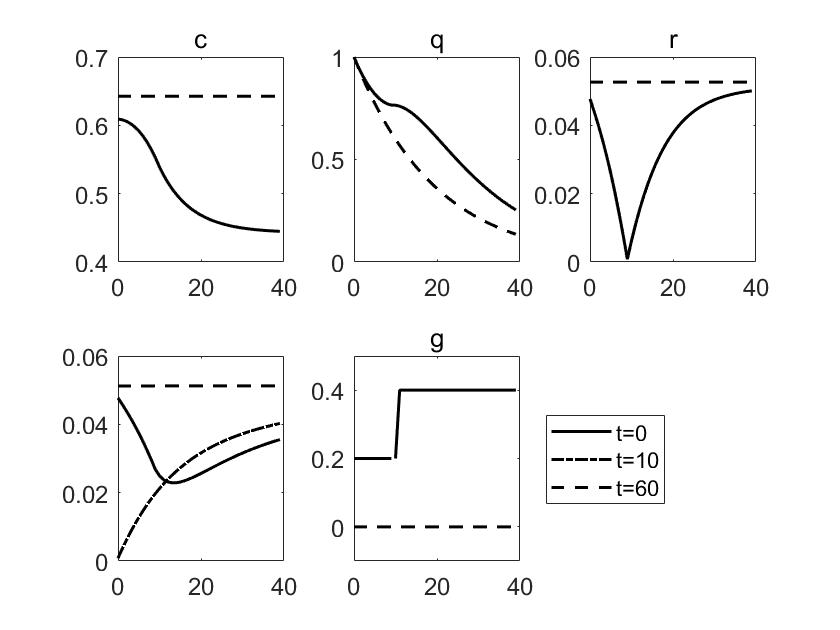
\includegraphics[width=0.8\linewidth]{fig17.jpg}
            \caption{Response to foreseen once-and-for-all increase in g at t = 10. Yield curves for t = 0 (solid line), t = 10
(dashdotted line) and t = 60 (dashed line); term to maturity is on the x axis for the yield curve, time for the other
panels}\label{17}
\end{figure}

\subsection{The model with elastic labor supply}

In this section we modify the previous model by allowing for elastic labor supply. Now the representative agent maximizes

$$\sum_{t=0}{\infty}\beta_tlogc_t+B(1-n_t)$$

where B is substantially greater than 1 to assure an interior solution $n \in (0,1)$ for labor supply.

Feasible allocations satisfy

$$g_t+c_t+k_{t+1}\le A_tk_t^{\alpha}n_t^{1-\alpha}+(1-\delta)k_t$$

The household budget constraint is

$$\sum_{t=0}{\infty}\{q_t(1+\tau_{c,t})+q_t[k_{t+1}-(1-\delta)k_t]\}\le\sum_{t=0}{\infty}q_t\{\eta_t(1-\tau_{k,t})k_t+w_t(1-\tau_{n,t})\}$$

The following conditions characterize the endogenous variables in the model equilibrium:

\begin{equation}\label{22}
    c_t=A_tk_t^{\alpha}n_t^{1-\alpha}+(1-\delta)k_t-k_{t+1}-g_t
\end{equation}
\begin{equation}\label{23}
    c_t^(-1)=\beta c_{t+1}^{-1}(\frac{1+\tau_{c,t}}{1+\tau_{c,t+1}})[(1-\delta)+(1-\tau_{k,t+1})A_t\alpha k_{t+1}^{\alpha-1}n_{t+1}^{1-\alpha}]
\end{equation}
\begin{equation}\label{24}
    Bc_t(1+\tau_{c,t})=(1-\tau_{n,t})[(1-\alpha)A_tk_t^{\alpha}n_t^{-\alpha}]
\end{equation}

\subsubsection{Elastic Labor supply : Unforseen once-and-for-all increase in g at t=0}

An unforeseen once-and-for-all increase in g to .2 at t = 0 (Figure 18).\\
\\

\%----------------------------------------------------------------\\
\% Experiment  : Unforseen increase in g at t=0\\
\%----------------------------------------------------------------\\
\\
\% This program replicates figure 11.9.1 from chapter 11 of RMT3 by Ljungqvist and Sargent\\
\\
\% Dynare records the endogenous variables with the following convention. Say N is the number of simulations(sample)\\
\%Index 1 : Initial values (steady sate)\\
\%Index 2 to N+1 : N simulated values\\
\%Index N+2 : Temnial Value (Steady State)\\
\% Warning:  we align c, k, and the taxes to exploit the dynare syntax. In Dynare the timing of the variable reflects the date\\
\%when the variable is decided. For instance the capital stock for time 't' is decided in time 't-1'(end of period). So a statement like\\
\% k(t+1) = i(t) + (1-del)*k(t) would translate to " k(t) = i(t) +(1-del)*k(t-1)" in the code.\\
\\
\%----------------------------------------------------------------\\
\% 1. Defining variables\\
\%----------------------------------------------------------------\\
\\
\%Declares the endogenous variables consumption ('c') capital stock (k);\\
var c k n;\\
\%declares the exogenous variables   consumption tax ('tauc'), capital tax('tauk'), government spending('g')\\
varexo tauc tauk taun g;\\
\\
parameters bet gam del alpha A B;\\
\\
\%----------------------------------------------------------------\\
\% 2. Calibration and alignment convention\\
\%----------------------------------------------------------------\\
\\
bet=.95;  \% discount factor\\
gam=1;    \% CRRA parameter\\
del=.2;  \% depreciation rate\\
alpha=.33; \%  capital's share\\
A=1;    \% productivity\\
B=3; \% coeffecient on leisure\\
\\
\% Alignment convention:\\
\% g tauc tauk taun are now columns of ex\_. Because of a bad design decision\\
\% the date of ex\_(1,:) doesn't necessarily match the date in endogenous variables. Whether they match depends\\
\% on the number of lag periods in endogenous versus exogenous variables.\\
\\
\% These decisions and the timing conventions mean that\\
\% k(1) records the initial steady state, while k(102) records the terminal steady state values.\\
\% For j > 1, k(j) records the variables for j-1th smimulation where the capital stock decision\\
\%taken in j-1 th simulation i.e stock at the begining of period j.\\
\% The variable ex\_ also follows a different timing convention i.e ex\_(j,:) records the value of exogenous variables in the j th simualtion.\\
\%The jump in the government policy is reflected in ex\_(10,1) for instance.\\
\\
\%----------------------------------------------------------------\\
\% 3. Model\\
\%----------------------------------------------------------------\\
\\
model;\\
\\
\%Feasibility\\
k=A*k(-1)\^alpha*n\^(1-alpha)+(1-del)*k(-1)-c-g;\\
\\
\%Euler equation\\
c\^(-gam)= bet*(c(+1)\^(-gam))*((1+tauc)/(1+tauc(+1)))*((1-del) + (1-tauk(+1))*alpha*A*k\^(alpha-1)*n(+1)\^(1-alpha));\\
\\
\%Consumption leisure choice\\
B/c\^(-gam)=(1-taun)*((1-alpha)*A*k(-1)\^(alpha)*n\^(-alpha))*(1+tauc)\^-1;\\
\\
end;\\
\\
\%----------------------------------------------------------------\\
\% 4. Computation\\
\%----------------------------------------------------------------\\
\\
initval;\\
k=1.5;\\
c=0.6;\\
g = .2;\\
n=1.02;\\
tauc = 0;\\
tauk = 0;\\
taun=0;\\
end;\\
steady; \% put this in if you want to start from the initial steady state, comment it out to start from the indicated values\\
\\
endval; \% The following values determine the new steady state after the shocks.\\
k=1.5;\\
c=0.6;\\
g =.4;\\
n=1.02;\\
tauc =0;\\
tauk =0;\\
taun=0;\\
end;\\
\\
steady; \% We use steady again and the enval provided are initial guesses for dynare to compute the ss.\\
\\
\% now solve the model\\
simul(periods=100);\\
\\
\% Compute the initial steady state for consumption to later do the plots.\\
c0=c(1);\\
k0 = k(1);\\
n0=n(1);\\
\% g is in ex\_(:,1) since it is stored in alphabetical order\\
g0 = .2;\\
\\
\%----------------------------------------------------------------\\
\% 5. Graphs and plots for other endogenous variables\\
\%----------------------------------------------------------------\\
\\
\%Let N be the periods to plot\\
N=40;\\
\\
\% The following equation compute the other endogenous variables use in the plots below\\
\% Since they are function of capital and consumption, so we can compute them from the solved\\
\% model above.\\
\% These equations were taken from page 371 of RMT3\\
rbig0=1/bet;\\
rbig=c(2:101).\^(-gam)./(bet*c(3:102).\^(-gam));\\
nq0=alpha*A*k0\^(alpha-1)*n0\^(1-alpha);\\
nq=alpha*A*k(1:100).\^(alpha-1).*(n(2:101).\^(1-alpha));\\
wq0=A*(1-alpha)*k0\^(alpha)*n0\^(-alpha);\\
wq=(1-alpha)*A*k(1:100).\^alpha.*(n(2:101).\^(-alpha));\\
\\
\%Now we plot the responses of the endogenous variables to the shock.\\
x=0:N-1;\\
figure(1)\\
\\
\% subplot for capital 'k'\\
subplot(2,3,1)\\
plot(x,[k0*ones(N,1)],'--k', x,k(1:N),'k','LineWidth',1.5) \% note the timing: we lag capital to correct for syntax\\
title('k','Fontsize',12)\\
set(gca,'Fontsize',12)\\
\\
\% subplot for consumption 'c'\\
subplot(2,3,2)\\
plot(x,[c0*ones(N,1)],'--k', x,c(2:N+1),'k','LineWidth',1.5)\\
title('c','Fontsize',12)\\
set(gca,'Fontsize',12)\\
\\
\% subplot for consumption 'n'\\
subplot(2,3,3)\\
plot(x,[n0*ones(N,1)],'--k', x,n(2:N+1),'k','LineWidth',1.5)\\
title('n','Fontsize',12)\\
set(gca,'Fontsize',12)\\
\\
\% subplot for cost of capital 'R\_bar'\\
subplot(2,3,4)\\
plot(x,[rbig0*ones(N,1)],'--k', x,rbig(1:N),'k','LineWidth',1.5)\\
title('$\verb|\|$overline{R}','interpreter', 'latex','Fontsize',12)\\
set(gca,'Fontsize',12)\\
\\
\% subplot for wage rate 'w'\\
subplot(2,3,5)\\
plot(x,[wq0*ones(N,1)],'--k', x,wq(1:N),'k','LineWidth',1.5)\\
title('w','Fontsize',12)\\
set(gca,'Fontsize',12)\\
\\
\% subplot for the experiment proposed\\
subplot(2,3,6)\\
plot(x,[g0*ones(N,1)],'--k', x,oo\_.exo\_simul(1:N,4),'k','LineWidth',1.5)\\
title('g','Fontsize',12)\\
axis([0 40 -.1 .5])\\
set(gca,'Fontsize',12)\\

\begin{figure}[htbp!]
		\centering
			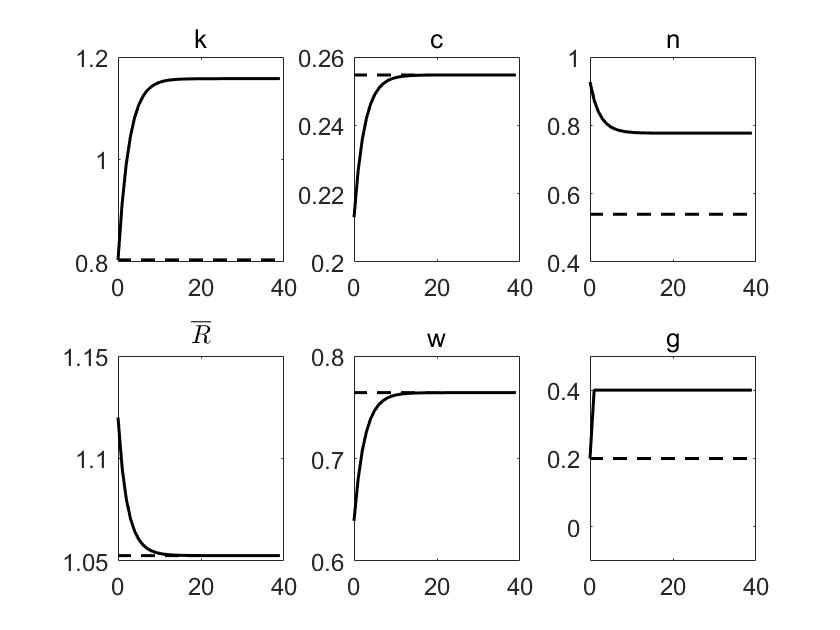
\includegraphics[width=0.8\linewidth]{fig18.jpg}
            \caption{Elastic labor supply: response to unforeseen increase in g at t = 0}\label{18}
\end{figure}

\subsubsection{Elastic Labor supply : Foreseen once-and-for-all increase in $\tau_n$ at t=0}

A foreseen once-and-for-all increase in $\tau_n$ to 20 percent at t = 0 (Figure 19).\\
\\
\textcolor{blue}{
initval;\\
k=1.5;\\
c=0.6;\\
g = .2;\\
n=1.02;\\
tauc = 0;\\
tauk = 0;\\
taun=0;\\
end;\\
steady;\\
endval;\\
k=1.5;\\
c=0.6;\\
g =.2;\\
n=1.02;\\
tauc =0;\\
tauk =0;\\
taun=0.2;\\
end;\\
steady;}\\

\begin{figure}[htbp!]
		\centering
			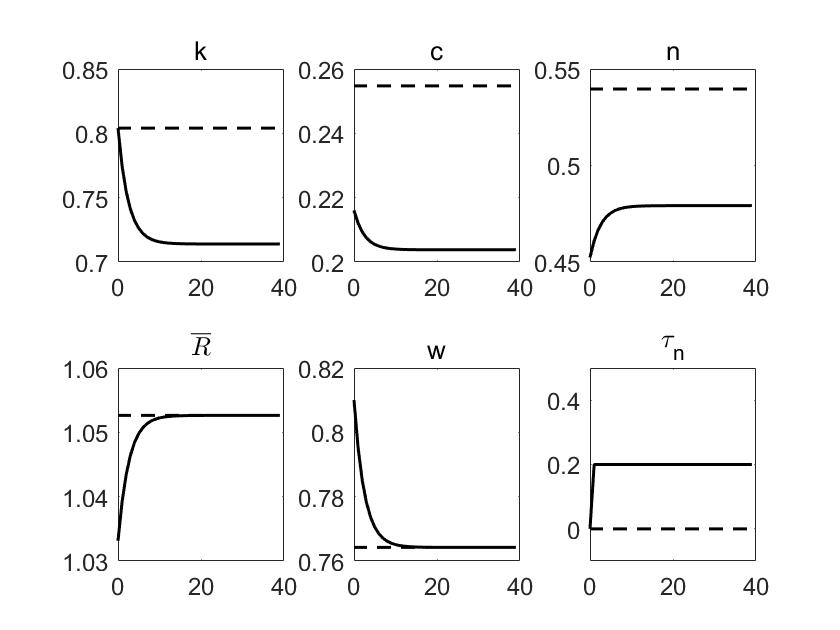
\includegraphics[width=0.8\linewidth]{fig19.jpg}
            \caption{Elastic labor supply: response to unforeseen increase in $\tau_n$ at t = 0}\label{10}
\end{figure}

\subsubsection{Elastic Labor supply : Foreseen once-and-for-all increase in $\tau_n$ at t=10}

A foreseen once-and-for-all increase in $\tau_n$ to 20 percent at t=10(Figure 20).\\
\\
\textcolor{blue}{
initval;\\
k=1.5;\\
c=0.6;\\
g = .2;\\
n=1.02;\\
tauc = 0;\\
tauk = 0;\\
taun=0;\\
end;\\
steady;\\
endval;\\
k=1.5;\\
c=0.6;\\
g =.2;\\
n=1.02;\\
tauc =0;\\
tauk =0;\\
taun=0.2;\\
end;\\
steady;\\
shocks;\\
var taun;\\
periods 1:10;\\
values 0;\\
end;}\\

\begin{figure}[htbp!]
		\centering
			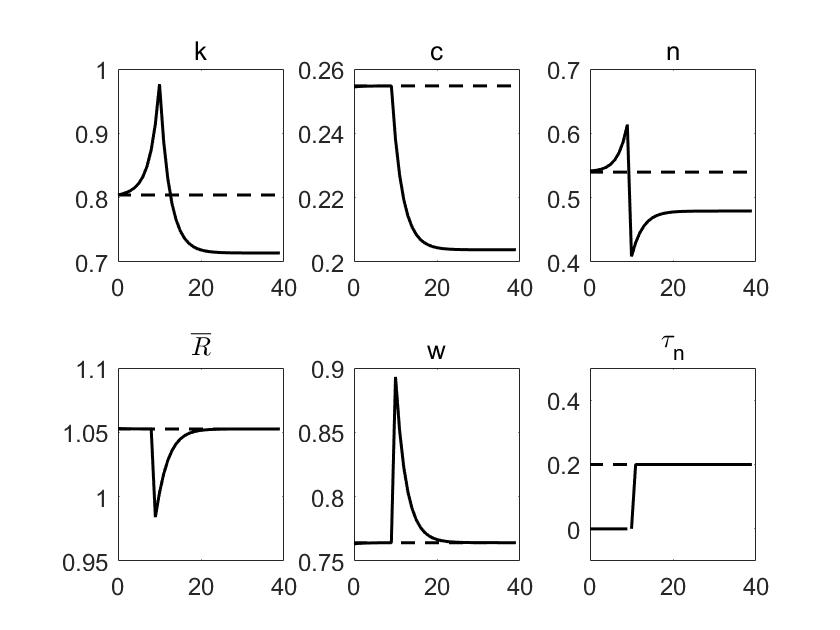
\includegraphics[width=0.8\linewidth]{fig20.jpg}
            \caption{Elastic labor supply: response to unforeseen increase in $\tau_n$ at t = 10}\label{20}
\end{figure}

\vspace{8cm}

\section{The demand for money during hyperinflations}

Sargent (1977) specified and estimated a joint stochastic process for money growth and inflation that was designed to make the adaptive expectations model of Cagan (1956) consistent with rational expectations. The model has the form

\begin{equation}\label{25}
    m_t-p_t=\alpha \pi_t+u_t
\end{equation}
\begin{equation}\label{26}
    \pi_t=\frac{1-\lambda}{1-\lambda L}(p_t-p_{t-1})=\frac{1-\lambda}{1-\lambda L}x_t
\end{equation}
\begin{equation}\label{27}
    \mu_t=m_t-m_{t-1}
\end{equation}

with $\alpha<0$, $m$ being the log of money supply, $\pi$ the expectation of inflation, $p$ the log of the price level and u an error term whose specification is described below. The hypothesis of rational expectations imposes

\begin{equation}\label{28}
    \pi_t=E_tx_{t+1}
\end{equation}

Sargent (1977) reverse engineered a process for xt such that Cagan’s adaptive expectations scheme is equal to rational expectations. The following conditions ensure the rationality of Cagan’s expectations scheme

\begin{equation}\label{29}
    u_t=u_{t-1}+\eta_t
\end{equation}
\begin{equation}\label{30}
    \mu_t=\frac{1-\lambda}{1-\lambda L}x_t+\epsilon_t
\end{equation}

$\eta$ and $\epsilon$ are both serially uncorrelated random error terms with mean zero and variances $\sigma_{\eta}^2$ and $\sigma_{\epsilon}^2$, respectively. For estimating the model, it is convenient to represent it in the following form

\begin{equation}\label{31}
\dbinom{x_t}{\mu_t}=\left(
\begin{matrix}
1 & 0 \\
1-\lambda & \lambda
\end{matrix}
\right) \dbinom{x_{t-1}}{\mu_{t-1}}+\dbinom{a_{1,t}}{a_{2,t}}-\lambda I\dbinom{a_{1,t-1}}{a_{2,t-1}}
\end{equation}

The a terms are linked to the random terms above via

\begin{equation}\label{32}
\dbinom{a_{1,t}}{a_{2,t}}=\left(
\begin{matrix}
1 & -1 \\
1+a(1-\lambda) & -(1-\lambda)
\end{matrix}
\right) (\lambda+(1-\lambda)\alpha))^{-1}\dbinom{\epsilon_{t}}{\eta_{t}}
\end{equation}

The code below estimates representation (31) by maximum likelihood:\\
\\
\textcolor{blue}{
\% this program estimates the model in\\
\% "The Demand for Money during Hyperinflations under Rational Expectations: I" by T. Sargent, IER 1977 using maximum likelihood\\
\% variables are defined as follows:\\
\% x=p\_t-p\_{t-1}, p being the log of the price level\\
\% mu=m\_t-m\_{t-1}, m being the log of money supply\\
\% note that in contrast to the paper eta and epsilon have variance 1 (they are multiplied by the standard deviations)\\
\\
var x mu a1 a2;\\
\\
varexo epsilon eta;\\
\\
parameters alpha lambda sig\_eta sig\_epsilon;\\
\\
lambda=.5921;\\
alpha=-2.344;\\
sig\_eta=.001;\\
sig\_epsilon=.001;\\
\\
model;\\
x=x(-1)-lambda*a1(-1)+(1/(lambda+alpha*(1-lambda)))*sig\_epsilon*epsilon-(1/(lambda+alpha*(1-lambda)))*sig\_eta*eta;\\
mu=(1-lambda)*x(-1)+lambda*mu(-1)-lambda*a2(-1)+(1+alpha*(1-lambda))/(lambda+alpha*(1-lambda))*sig\_epsilon*epsilon-(1-lambda)/(lambda+alpha*(1-lambda))*sig\_eta*eta;\\
a1=(1/(lambda+alpha*(1-lambda)))*sig\_epsilon*epsilon-(1/(lambda+alpha*(1-lambda)))*sig\_eta*eta;\\
a2=(1+alpha*(1-lambda))/(lambda+alpha*(1-lambda))*sig\_epsilon*epsilon-(1-lambda)/(lambda+alpha*(1-lambda))*sig\_eta*eta;\\
end;\\
\\
steady;\\
\\
shocks;\\
\\
var eta;\\
stderr 1;\\
var epsilon;\\
stderr 1;\\
end;\\
\\
estimated\_params;\\
\% ML estimation setup\\
\% parameter name, initial value, boundaries\_low, ...\_up;\\
lambda, .5, 0.25, 0.75;\\
alpha, -2, -8, -0.1;\\
sig\_eta, .0001, 0.0001, 0.3;\\
sig\_epsilon, .0001, 0.0001, 0.3;\\
end;\\
\\
varobs mu x;\\
\\
estimation(datafile=cagan\_data,first\_obs=1,nobs=34,mh\_replic=0,mode\_compute=4,mode\_check,diffuse\_filter);}\\

The data for the estimation are from Cagan (1956) for Germany\footnote{The data are demeaned, allowing us to ignore constant terms in the model}. The shape of the log-likelihood function is plotted in figure 21.

\begin{figure}[htbp!]
		\centering
			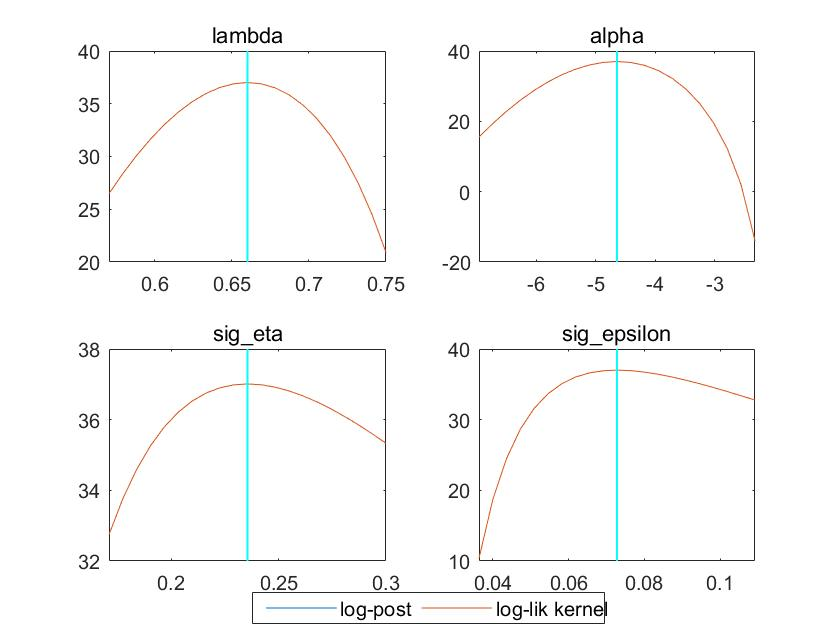
\includegraphics[width=0.8\linewidth]{fig21.jpg}
            \caption{the Log-Likelihood function for the hyperinflation model}\label{21}
\end{figure}

\begin{table}{h}
\centering
\caption{Results from Maximum likelihood}\label{6}
\begin{tabular}{cccc}
\hline
Parameter&Estimate&s.d.&t-stat.\\
\hline
$\lambda$&0.6601&0.0542&12.1709\\
$\alpha$&-4.6436&2.8468&1.6312\\
$\sigma_{\eta}$&0.2355&0.1992&1.1824\\
$\sigma_{\epsilon}$&0.0728&0.0101&7.2353\\
\hline
\end{tabular}
\end{table}

\vspace{4cm}

Next we estimate this model using Bayesian techniques. For this we replace the last part of the code above with\\
\\
\textcolor{blue}{
estimated\_params;\\
\% Bayesian setup\\
lambda, uniform\_pdf, 0.68, .5;\\
alpha, uniform\_pdf, -5, 2;\\
sig\_eta,uniform\_pdf, .5, 0.25;\\
sig\_epsilon, uniform\_pdf, .5, 0.25;\\
end;\\
\\
varobs mu x;\\
\\
estimation(datafile=cagan\_data,nobs=34,mh\_replic=25000,mh\_nblocks=1,mh\_jscale=1,mode\_compute=4,diffuse\_filter);}\\

Note that the priors we have chosen are reasonably loose, but given that there are only 34 observations we have opted to use somewhat informative priors. The posteriors and priors are plotted in figure 22.

\begin{figure}[htbp!]
		\centering
			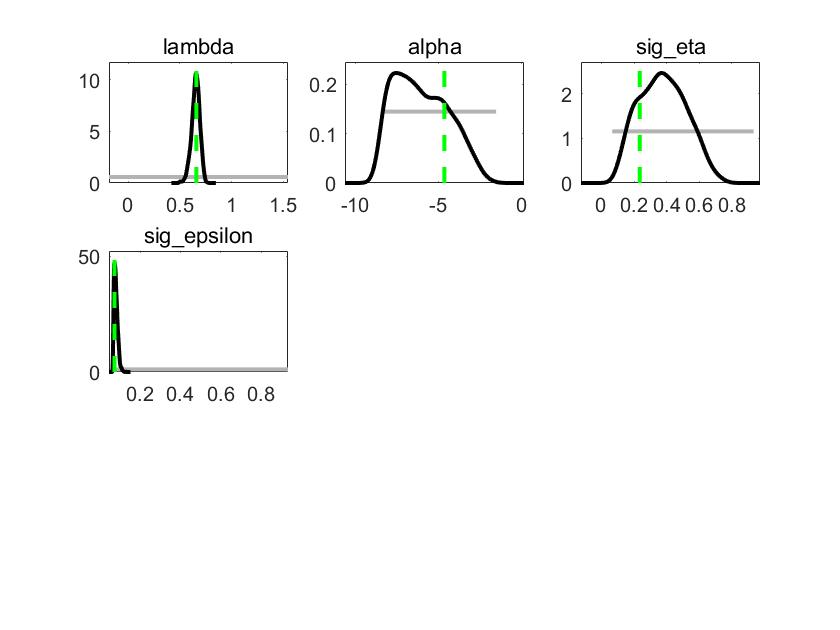
\includegraphics[width=0.8\linewidth]{fig22.jpg}
            \caption{Posteriors and priors for the hyperinflation model}\label{22}
\end{figure}



\section{Solving and estimating Hall’s permanent income model}

This note describes a suite of Dynare programs to simulate and estimate the permanent income model of Hall(1988).

\subsection{The model}

A consumer faces the following decision problem:

$$\underbrace{max}_{c_t,k_t}~-\frac{1}{2}\sum_{t=0}{\infty}\beta^t(c_t-b_t)^2$$

subject to the following constraints

$$c_t+k_t=R_tk_{t-1}+d_t$$
$$d_t=\rho d_{t-1}+(1-\rho)\mu_d+\epsilon_d$$
$$b_t=\rho_bb_{t-1}+(1-\rho_b)\mu_b+\epsilon_b$$

We assume that $\beta R=1$ and that there is no depreciation, which leads to the following law of motion for investment:

$$i_t=k_t-k_{t-1}$$

From the Lagrangian for this problem one obtains the following first order conditions:

$$\mu_{c,t}=\mu_{c,t+1}$$
$$\mu_{c,t}=b_t+c_t$$

where $\mu_{c,t}$ is the marginal utility of consumption or the Lagrange multiplier.

Note that this problem has a unit root and so there exist no steady state. However, we can supply ONE solution corresponding to an initial k that we give to Dynare.

The following Dynare code simulates data from this model:\\
\\
\textcolor{blue}{
var c k mu\_c b d in;\\
varexo e\_d e\_b;\\
\\
parameters R rho rho\_b mu\_b mu\_d;\\
R=1.05;\\
\% rho=0.9;\\
rho = 0;\\
mu\_b=30;\\
mu\_d=5;\\
rho\_b = 0;\\
\\
model(linear);\\
\\
 c+k = R*k(-1) + d;\\
 mu\_c = b - c;\\
 mu\_c=mu\_c(+1);\\
 d= rho*d(-1)+ mu\_d*(1-rho) + e\_d;\\
 b=(1-rho\_b)*mu\_b+rho\_b*b(-1)+e\_b;\\
 in = k - k(-1);\\
 end;\\
\\
\%With a unit root, there exists no steady state.  Use the following trick.\\
\%Supply ONE solution corresponding to the initial k that you named.\\
\\
initval;\\
d=mu\_d;\\
k=100;\\
c = (R-1)*k +d;\\
mu\_c=mu\_b-c;\\
b=mu\_b;\\
end;\\
\\
shocks;\\
var e\_d;\\
stderr 1;\\
var e\_b;\\
stderr 1;\\
end;\\
\\
steady;\\
check;\\
\\
stoch\_simul(order=1, periods=500, irf=10);\\
save data\_hall c in;}\\

\begin{figure}[htbp!]
		\centering
			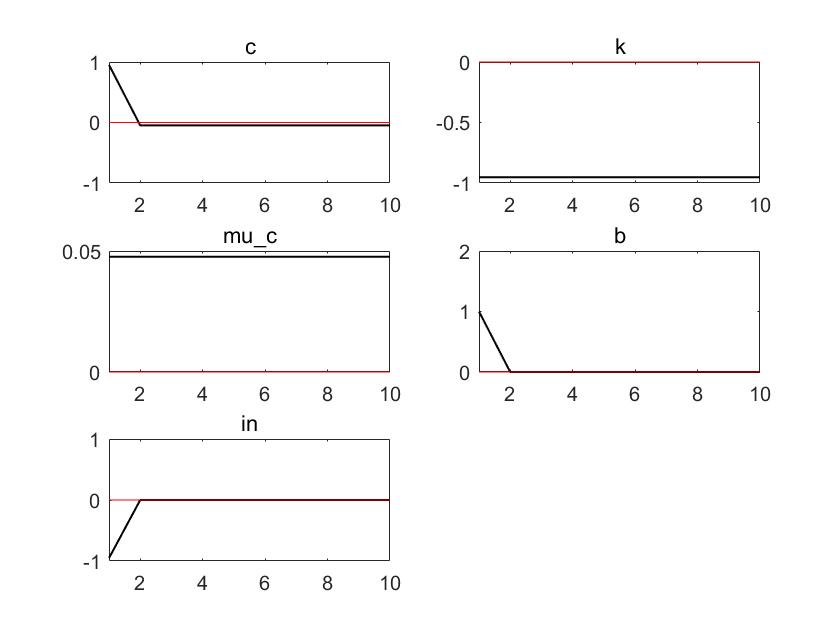
\includegraphics[width=0.8\linewidth]{fig23.jpg}
            \caption{A shock to $\epsilon_b$}\label{23}
\end{figure}

Next, we proceed to estimate a subset of the parameters of the model by ML using simulated data obtained from the previous code. To do so we add the following few lines of code. Notice how we use the command unit root vars to initialize the Kalman filter with a diffuse prior. We do this because k is not stationary – Hall’s model with $\beta R=1$ has a solution for k that has a unit root and that is co-integrated with consumption.\\
\\
\textcolor{blue}{
estimated\_params;\\
\% ML estimation setup\\
\% parameter name, initial value, boundaries\_low, ...\_up;\\
rho, 0.9, 0, 1;\\
R, 1.05, 0, 1.5;\\
end;\\
varobs c in;\\
\\
estimation(datafile=data\_hall,first\_obs=101,nobs=200,mh\_replic=0,mode\_compute=4,mode\_check,diffuse\_filter);}\\

\begin{figure}[htbp!]
		\centering
			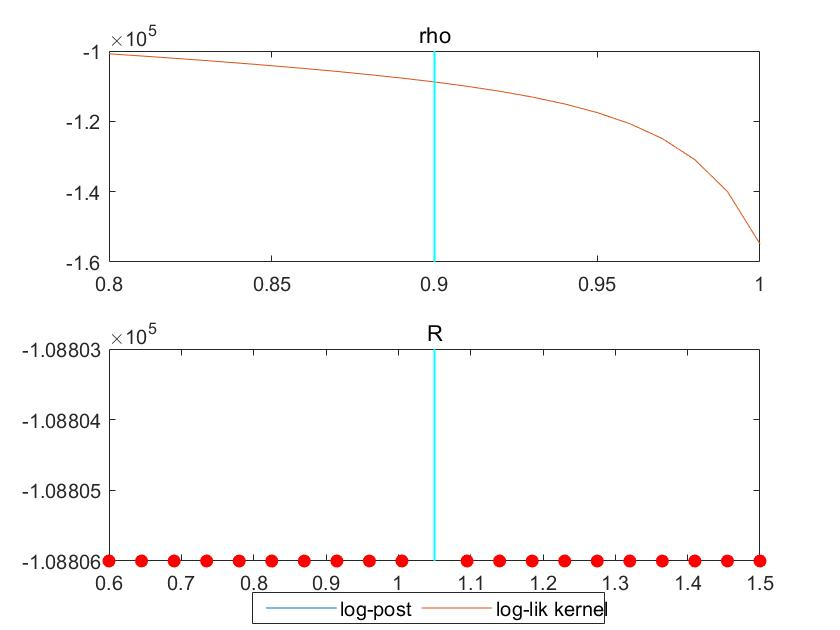
\includegraphics[width=0.8\linewidth]{fig24.jpg}
            \caption{priors and posteriors from the ML estimation of Hall’s model}\label{24}
\end{figure}

We proceed to estimate the same subset of the parameters using Bayesian techniques: This is implemented in Dynare by adding the following few lines of code.\\
\\
\textcolor{blue}{
estimated\_params;\\
rho,beta\_pdf, 0.1, 0.2;\\
R,norm\_pdf, 1.02, 0.05;\\
end;\\
varobs c in;\\
\\
estimation(datafile=data\_hall,first\_obs=101,nobs=200,mode\_compute=6,mh\_replic=1000,mh\_nblocks=2,mh\_jscale=2,diffuse\_filter);}\\



\section{Solving and estimating Ryoo and Rosen’s (2004) model of the market for engineers}

This section describes a suite of Dynare programs to simulate and estimate a model of Aloysius Siow (1984) and Jaewoo Ryoo and Sherwin Rosen (2004) of the labor market for engineers.

\subsection{The model}

Ryoo and Rosen studied a partial equilibrium model determining a stock of ’engineers’ Nt; the number of new entrants into engineering school, st; and the wage level wt of engineers.\footnote{Sherwin Rosen showed this version of the model to Sargent in Chicago in fall 1995.} It takes k periods of schooling to become an engineer. The model consists of the following components:

The present value of wages of an engineer:

$$P_t=(1-\delta)\beta P_{t+1}+(1-\delta)^k\beta^kw_{t+k}$$

A supply of new engineering students:

$$s_t=a_0+a_1P_t+e_{s,t}$$

A time-to-build structure of the education process:

$$N_t=(1-\delta)N_{t-1}+s_{t-k}$$

A demand curve for engineers:

$$N_t=d_0-d_1w_t+e_{d,t}$$

The following Dynare code simulates data from this model:\\
\\
\textcolor{blue}{
\% Rosen schooling model\\
\% The model is the one Sherwin Rosen showed Sargent in Sargent's Chicago office.\\
\% The equations are\\
\\
\%  s\_t = a0 + a1*P\_t + e\_st   ;  flow supply of new engineers\\
\%  N\_t = (1-delta)*N\_{t-1} + s\_{t-k} ;  time to school engineers\\
\%  N\_t = d0 - d1*W\_t +e\_dt ; demand for engineers\\
\%  P\_t = (1-delta)*bet P\_(t+1) + beta\^k*W\_(t+k);  present value of wages of an engineer\\
\\
var s N P W;\\
varexo e\_s e\_d;\\
\\
parameters a0 a1 delta d0 d1  bet k;\\
a0=10;\\
a1=1;\\
d0=1000;\\
d1=1;\\
bet=.99;\\
delta=.02;\\
\\
model(linear);\\
s=a0+a1*P+e\_s;  \% flow supply of new entrants\\
N=(1-delta)*N(-1) + s(-4); \% evolution of the stock\\
N=d0-d1*W+e\_d;  \% stock demand equation\\
P=bet*(1-delta)*P(+1) + bet\^4*(1-delta)\^4*W(+4); \% present value of wages\\
end;\\
\\
initval;\\
s=0;\\
N=0;\\
P=0;\\
W=0;\\
end;\\
\\
shocks;\\
var e\_d;\\
stderr 1;\\
var e\_s;\\
stderr 1;\\
end;\\
\\
steady;\\
check;\\
\\
stoch\_simul(order=1, periods=500, irf=10);\\
save data\_rosen s N P W;}\\

Figure 25 plots the response of endogenous variables to $\epsilon_{s}$.

\begin{figure}[htbp!]
		\centering
			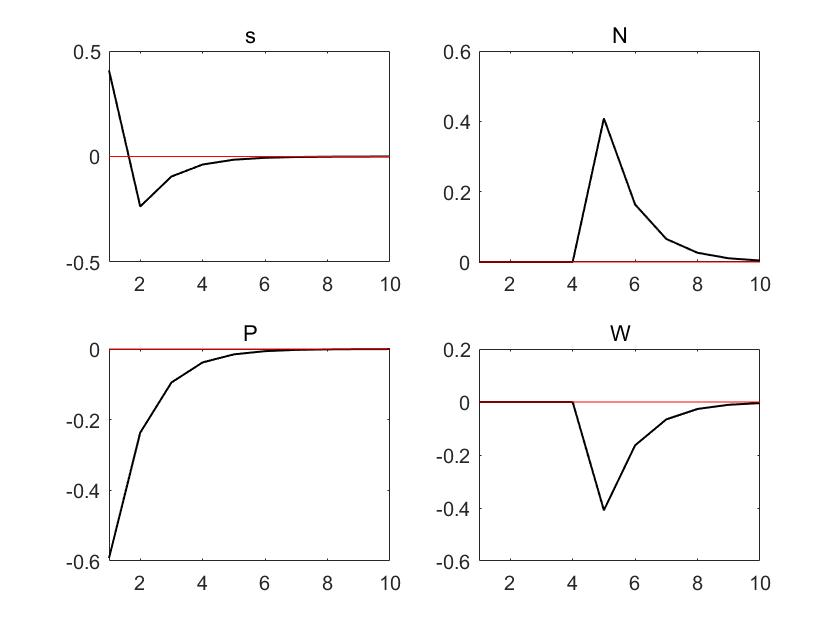
\includegraphics[width=0.8\linewidth]{fig26.jpg}
            \caption{A shock to $\epsilon_{s,t}$}\label{26}
\end{figure}

\vspace{4cm}

Note that in this code we set k = 4. Dynare does not let you use a parameter as lag length.

Next, we estimate a subset of the parameters of the model by ML using simulated data obtained from the previous code. To do so we add the following lines of code.\\
\\
\textcolor{blue}{
estimated\_params;\\
a1, .5, -10, 10;\\
d1, .5, -20, 40;\\
stderr e\_d, .5, .05, 5;\\
stderr e\_s, .3, .05, 6; \\
end;\\
\% these are the ranges for the parameters\\
varobs W N;\\
estimation(datafile=data\_rosen,first\_obs=101,nobs=200,mh\_replic=0,mode\_compute=4,mode\_check);}\\

Figure 26 plots the log-likelihood function for the parameters.

\begin{figure}[htbp!]
		\centering
			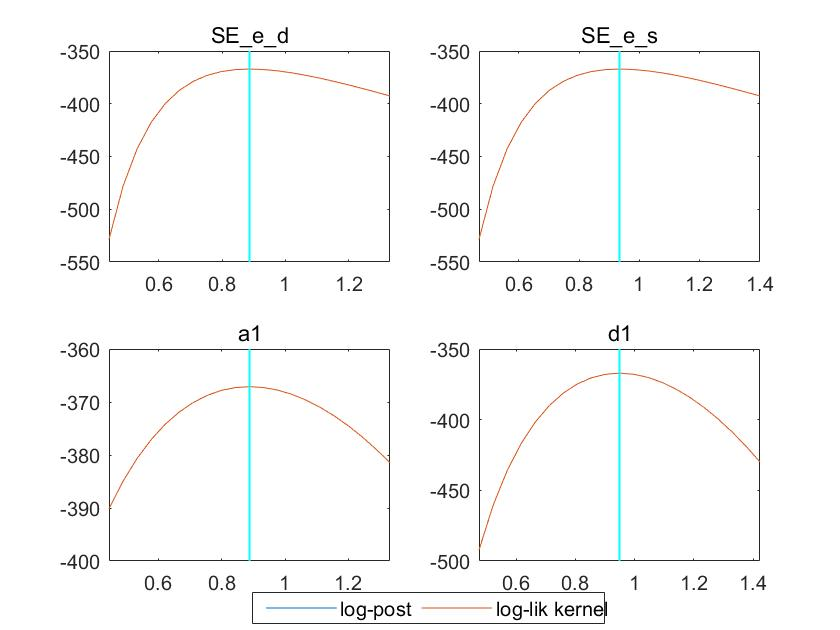
\includegraphics[width=0.8\linewidth]{fig27.jpg}
            \caption{the Log-Likelihood for Ryoo and Rosen’s model}\label{27}
\end{figure}

\vspace{4cm}

We proceed to estimate the same subset of the parameters using Bayesian techniques. We implemented this in Dynare by adding the following lines of code.\\
\\
\textcolor{blue}{
estimated\_params;\\
a1, gamma\_pdf, .5, .5;\\
d1, gamma\_pdf, 2, .5;\\
stderr e\_d,inv\_gamma\_pdf,.5, 30;\\
stderr e\_s,inv\_gamma\_pdf,.2, 30;\\
\% The syntax for to input the priors is the following:\\
\% variable name, prior distribution, parameters of distribution.\\
end;\\
varobs W N;\\
estimation(datafile=data\_rosen,first\_obs=101,nobs=200,mh\_replic=10000,mh\_nblocks=2,
mh\_jscale=2,mode\_compute=0,mode\_file=rosenestimateML\_mode);}\\

\begin{figure}[htbp!]
		\centering
			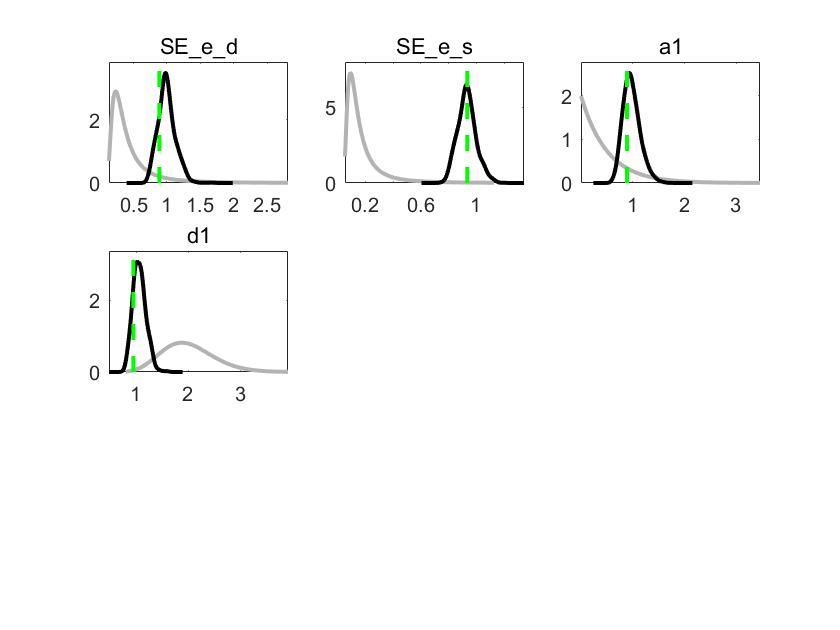
\includegraphics[width=0.8\linewidth]{fig28.jpg}
            \caption{the Log-Likelihood for Ryoo and Rosen’s model}\label{28}
\end{figure}

\begin{table}{h}
\centering
\caption{Results from Bayesian Estimation}\label{7}
\begin{tabular}{lcccccc}
\hline
Parameter&Prior mean&Posterior mean&90\% HPD&interval&Prior&pst.dev.\\
\hline
$a_1$&0.500&0.9753&0.7429&1.2383&gamm&0.5000\\
$d_1$&2.000&1.0638&0.8841&1.2800&gamm&0.5000\\
$\epsilon_d$&0.500&0.9945&0.7655&1.1704&invg&30.0000\\
$\epsilon_s$&0.200&0.9306&0.8120&1.0245&invg&30.0000\\
\hline
\end{tabular}
\end{table}

\vspace{4cm}

\section{Estimation of Bansal and Yaron(2004) consumption growth process}

Let consumption growth have the state space representation

$$x_t=\rho x_{t-1}+\sigma_x\epsilon_{x,t}$$
$$\Delta c_t=\mu_{c}+x_{t-1}+\sigma_c\epsilon_{c,t}$$

where the shocks $\epsilon_{c,t}$ and $\epsilon_{x,t}$ are i.i.d. standard normal. We use quarterly growth rate of per capita U.S. consumption over the period 1947.2-2003.3 to estimate the four unknown parameters. The following Dynare code does this by maximum likelihood.\\
\\
\textcolor{blue}{
var x y;\\
varexo e\_x e\_u;\\
\\
parameters  rho sig\_x sig\_u mu\_y;\\
\\
rho = .98;\\
mu\_y=.015;\\
sig\_x=0.00025;\\
sig\_u=.0078;\\
\\
model(linear);\\
x=rho*x(-1) + sig\_x*e\_x;\\
y=mu\_y + x(-1) + sig\_u*e\_u;\\
end;\\
\\
initval;\\
x=0;\\
y=mu\_y;\\
end;\\
\\
steady;\\
\\
shocks;\\
var e\_x;\\
stderr 1;\\
var e\_u;\\
stderr 1;\\
end;\\
\\
estimated\_params;\\
\% ML estimation setup\\
\% parameter name, initial value, boundaries\_low, ...\_up;\\
 rho, 0, -0.99, 0.999;  \% use this for unconstrained max likelihood\\
\% rho, .98, .975, .999 ;  \% use this for long run risk model\\
\% sig\_x, .0004,.0001,.05 ; \% use this for the long run risk model\\
sig\_x, .0005, .00000000001, .01;  \% use this for unconstrained max likelihood\\
sig\_u, .007,.001, .1;\\
mu\_y, .014, .0001, .04;\\
\\
end;\\
\\
varobs y;\\
estimation(datafile=data\_consRicardoypg,first\_obs=1,nobs=227,mh\_replic=0,mode\_compute=4,mode\_check);}\\

Table 10 reports the estimated parameter from Dynare.

\vspace{12cm}

\begin{table}{h}
\centering
\caption{Results from Maximum likelihood}\label{10}
\begin{tabular}{cccc}
\hline
Parameter&Estimate&s.d.&t-stat.\\
\hline
$\rho$&0.5623&0.1926&2.9195\\
$\mu_y$&0.0056&0.0005&10.7599\\
$\sigma_x$&0.0030&0.0011&2.6935\\
$\sigma_u$&0.0040&0.0007&5.4546\\
\hline
\end{tabular}
\end{table}


Figure 29 also plots the log-likelihood function along several dimensions.

\begin{figure}[htbp!]
		\centering
			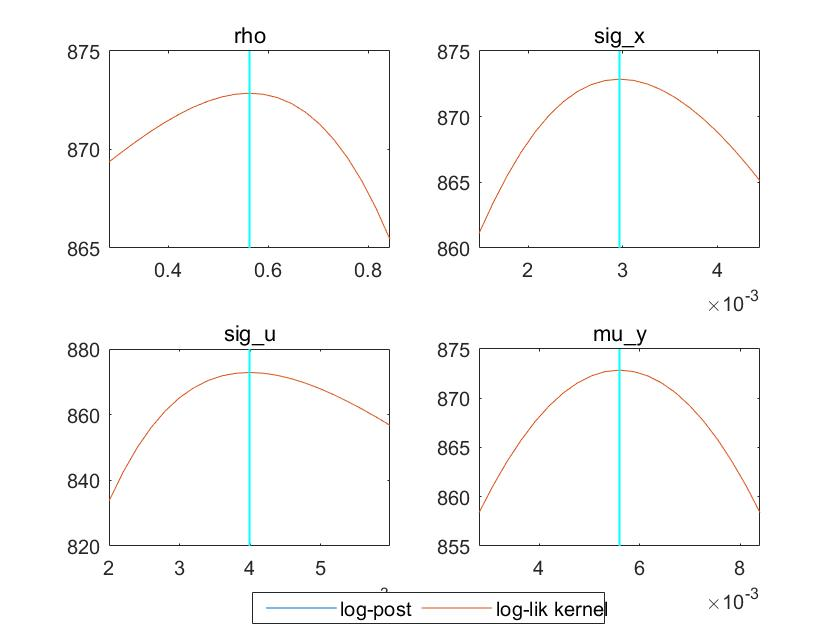
\includegraphics[width=0.8\linewidth]{fig29.jpg}
            \caption{the Log-Likelihood function for the consumption growth model}\label{29}
\end{figure}

Next, we estimate the same model using Bayesian techniques and two different sets of priors. The first set of priors are tight around the calibrated values used in Bansal and Yaron (2004). To accomplish this, we can simply change the following lines of code from our MLE program above.\\
\\
\textcolor{blue}{
estimated\_params;\\
rho, beta\_pdf, .98, .01;\\
mu\_y, uniform\_pdf, .005, .0025;\\
sig\_u, inv\_gamma\_pdf, .003, inf;\\
sig\_x, inv\_gamma\_pdf, .003, inf;\\
\% The syntax for to input the priors is the following:\\
\% variable name, prior distribution, parameters of distribution.\\
end;\\
varobs y;\\
estimation(datafile=data\_consRicardoypg,first\_obs=1,nobs=227,mh\_replic=5000,mh\_nblocks=1,mh\_jscale=1);}\\
\\

Table 11 reports the estimated parameter from Dynare.

\begin{table}
\centering
\caption{Results from Bayesian Estimation}\label{11}
\begin{tabular}{lcccccc}
\hline
Parameter&Prior mean&Posterior mean&90\% HPD&interval&Prior&pst.dev.\\
\hline
$\rho$&0.980&0.9711&0.9513&0.9905&beta&0.0100\\
$\mu_y$&0.005&0.0051&0.0019&0.0088&unif&0.0025\\
$\sigma_u$&0.003&0.0048&0.0043&0.0053&invg&Inf\\
$\sigma_x$&0.003&0.0012&0.0007&0.0016&invg&Inf\\
\hline
\end{tabular}
\end{table}


Figure 29 plots the prior and the posterior densities for the estimated parameters. The posteriors are plotted in black and priors in gray. A vertical green line denotes a posterior mean.

\begin{figure}[htbp!]
		\centering
			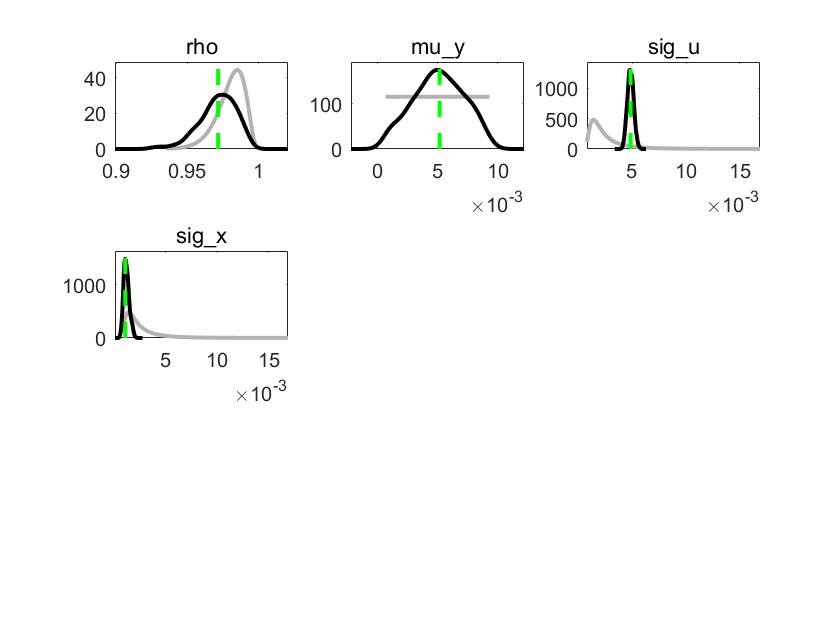
\includegraphics[width=0.8\linewidth]{fig30.jpg}
            \caption{Prior and Posteriors for the Bansal and Yaron (2004) endownment process}\label{30}
\end{figure}

Next, we set vague priors for $\rho$ and for $\mu_y$.\\
\\
\textcolor{blue}{
rho, beta\_pdf, .5, .2;\\
mu\_y, uniform\_pdf, .005, .0025;\\
sig\_u, inv\_gamma\_pdf, .003, inf;\\
sig\_x, inv\_gamma\_pdf, .003, inf;}\\

Table 12 reports the estimated parameter from Dynare.

\begin{table}{h}
\centering
\caption{Results from Bayesian Estimation}\label{12}
\begin{tabular}{lcccccc}
\hline
Parameter&Prior mean&Posterior mean&90\% HPD&interval&Prior&pst.dev.\\
\hline
$\rho$&0.500&0.5044&0.2604&0.7198&beta&0.0200\\
$\mu_y$&0.004&0.0056&0.0046&0.0064&unif&0.003\\
$\sigma_u$&0.003&0.0035&0.0015&0.0048&invg&Inf\\
$\sigma_x$&0.003&0.0034&0.0020&0.0053&invg&Inf\\
\hline
\end{tabular}
\end{table}

Figure 30 plots the prior and the posterior densities for the estimated parameters. Notice that with a more diffuse prior on $\rho$, the posteriors for $\mu_y$ are tighter.

\begin{figure}[htbp!]
		\centering
			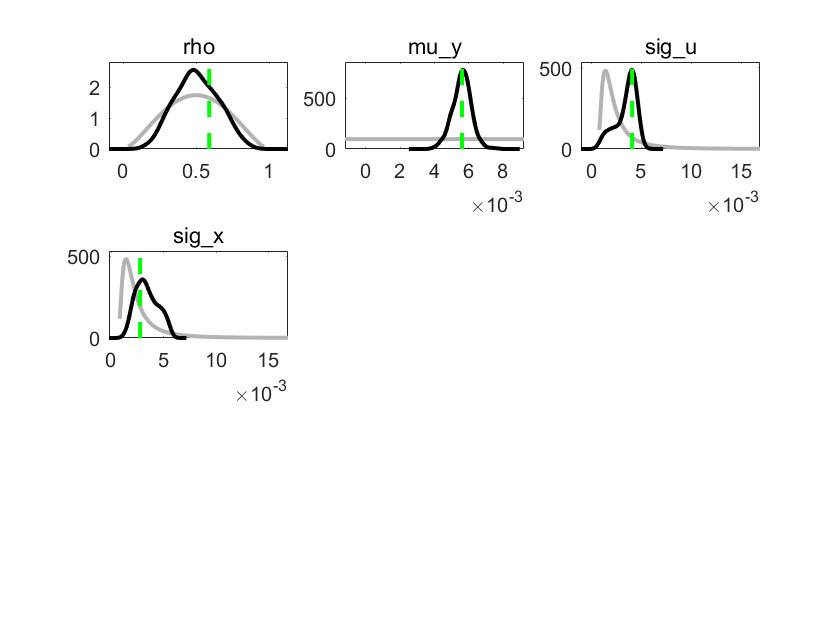
\includegraphics[width=0.8\linewidth]{fig31.jpg}
            \caption{Prior and Posteriors for the Bansal and Yaron (2004) endownment process}\label{31}
\end{figure}

\section{Robust permanent income and pricing}

Hansen, Sargent, and Tallarini (1999) study consumption, saving, and security market prices in a permanent income
model in which the agents mistrust their specification of the economic environment. The preferences of a representative consumer are defined in terms of the following risk-sensitivity recursion:

\begin{equation}\label{33}
U_t=u_t+\beta R_t(U_{t+1})
\end{equation}
\begin{equation}\label{34}
R_t(U_{t+1})=\frac{2}{\sigma}log[exp(\frac{\sigma U_{t+1}}{2})]
\end{equation}

with $u_t$ being the per-period utility function. Note that $\sigma=0$ corresponds to Von Neumann-Morgenstern preferences. The authors use a linear quadratic framework described below. Furthermore, they show that for a given $(\beta,\sigma)$ pair there exists another pair $(\hat{\beta},0)$ that gives the same equilibrium quantities. This observation simplifies solution and estimation of the model significantly. For the $\sigma=0$ case and HST’s linear-quadratic habit persistence model, preferences become

\begin{equation}\label{35}
U_0=E_0\sum_{t=0}{\infty}\beta^t(-(s_t-b)^2)
\end{equation}

with b being a subsistence point and s defined as

\begin{equation}\label{36}
s_t=(1+\lambda)c_t-\lambda h_{t-1}
\end{equation}
\begin{equation}\label{37}
h_t=\delta_hh_{t-1}+(1-\delta_h)c_t
\end{equation}

where $c_t$ is current period consumption and $h_{t-1}$ the habit stock. There is a linear production technology:

\begin{equation}\label{38}
c_t+i_t=\gamma k_{t-1}+d_t
\end{equation}
\begin{equation}\label{39}
k_t=\delta_k k_{t-1}+i_t
\end{equation}
\begin{equation}\label{40}
d_t=\mu_d+\hat{d}_t+\bar{d}_t
\end{equation}
\begin{equation}\label{41}
\bar{d}_t=(\phi_1+\phi_2)\bar{d}_{t-1}-\phi_1\phi_2\bar{d}_{t-2}+c_{\bar{d}}e_{1,t}
\end{equation}
\begin{equation}\label{42}
\hat{d}_t=(\alpha_1+\alpha_2)\hat{d}_{t-1}-\alpha_1\alpha_2\hat{d}_{t-2}+c_{\hat{d}}e_{2,t}
\end{equation}

$e_{1,t}$ and $e_{2,t}$ are standard normal iid shocks. Finally, we define the gross return on capital as

\begin{equation}\label{43}
R\equiv \delta_k+\gamma
\end{equation}

and impose

\begin{equation}\label{44}
R\beta=1
\end{equation}

To solve the planning problem, we formulate a Lagrangian with multipliers $2\beta^t\mu_{s,t}$ on (36), $2\beta^t\mu_{s,t}$ on (37) and $2\beta^t\mu_{h,t}$ on (38) (after substituting for investment $i_t$). The first order necessary conditions are:

\begin{equation}\label{45}
\mu_{s,t}=b-s_t
\end{equation}
\begin{equation}\label{46}
\mu_{c,t}=(1+\lambda)\mu_{s,t}+(1-\delta_h)\mu{h,t}
\end{equation}
\begin{equation}\label{47}
\mu{h,t}=\beta E_t[\delta_h\mu_{h,t+1}-\lambda \mu_{s,t+1}]
\end{equation}
\begin{equation}\label{48}
\mu_{c,t}=\mu_{c,t+1}
\end{equation}

plus (36)-(39). The following code estimates the model using maximum likelihood:\\
\\
\textcolor{blue}{
\% Estimates the Hansen Sargent and Tallarini model by maximum likelihood.\\
\\
var s c h k i d dhat dbar mus muc muh gamma R;\\
varexo e\_dhat e\_dbar;\\
\\
parameters lambda deltah deltak mud b bet phi1 phi2 cdbar alpha1 alpha2 cdhat;\\
bet=0.9971;\\
deltah=0.682;\\
lambda=2.443;\\
alpha1=0.813;\\
alpha2=0.189;\\
phi1=0.998;\\
phi2=0.704;\\
mud=13.710;\\
cdhat=0.155;\\
cdbar=0.108;\\
b=32;\\
deltak=0.975;\\
\\
model(linear);\\
R=deltak+gamma;\\
R*bet=1;\\
s=(1+lambda)*c-lambda*h(-1);\\
h=deltah*h(-1)+(1-deltah)*c;\\
k=deltak*k(-1)+i;\\
c+i=(1/bet-deltak)*k(-1)+d;\\
mus=b-s;\\
muc=(1+lambda)*mus+(1-deltah)*muh;\\
muh=bet*(deltah*muh(+1)-lambda*mus(+1));\\
muc=muc(+1);\\
d=mud+dbar+dhat;\\
dbar=(phi1+phi2)*dbar(-1) - phi1*phi2*dbar(-2) + cdbar*e\_dbar;\\
dhat=(alpha1+alpha2)*dhat(-1) - alpha1*alpha2*dhat(-2) + cdhat*e\_dhat;\\
end;\\
\\
initval;\\
R=1/bet;\\
gamma=R-deltak;\\
d=mud;\\
k=100;\\
i=(1-deltak)*k;\\
c=gamma*k+d-i;\\
h=c;\\
s=c;\\
mus=b-s;\\
muh=lambda/(deltah-1/bet)*mus;\\
muc=(1+lambda)*mus+(1-deltah)*muh;\\
end;\\
\\
steady(nocheck);\\
\\
shocks;\\
var e\_dhat;\\
stderr 1;\\
var e\_dbar;\\
stderr 1;\\
end;\\
\\
\% stoch\_simul(irf=0, periods=500);\\
\% save dataHST c i;\\
\\
estimated\_params;\\
bet, .9971, 0, .99999;\\
deltah, 0.682, 0.1, 0.8;\\
lambda, 2.443, 0.1, 50;\\
alpha1, 0.813, 0.6, 0.99999;\\
alpha2, 0.189, 0.01, 0.5;\\
phi1, 0.998, 0, 0.99999;\\
phi2, 0.704, 0, 0.9;\\
mud, 13.710, 1, 50;\\
cdhat, 0.155, 0.05, 0.2;\\
cdbar, 0.108, 0.05, 0.2;\\
end;\\
\\
varobs c i;\\
estimation(datafile=dataHST,first\_obs=1,nobs=500,mode\_compute=4,mode\_check,diffuse\_filter);}\\

To estimate the model using Bayesian techniques simply replace the last part of the code with\\
\\
\textcolor{blue}{
estimated\_params;\\
bet,uniform\_pdf, .9499999999, 0.0288675134306;\\
deltah,uniform\_pdf, 0.45, 0.202072594216;
lambda,uniform\_pdf,25.05,14.4048892163;
alpha1,uniform\_pdf, 0.8, 0.115470053809;
alpha2,uniform\_pdf, 0.25, 0.144337567297;
phi1,uniform\_pdf,0.8,0.115470053809;
phi2,uniform\_pdf, 0.5, 0.288675134595;
mud,uniform\_pdf, 24.5, 14.1450815951;
cdhat,uniform\_pdf,0.175,0.0721687836487;
cdbar,uniform\_pdf, 0.175, 0.0721687836487;\\
end;\\
\\
varobs c i;\\
estimation(datafile=dataHST,nobs=500,mode\_check,mh\_replic=10000,mh\_nblocks=1,mh\_jscale=0.2);}\\

The maximization routine used here (mode compute=4) is Chris Sims’ csminwel. Note that this procedure uses a random number generator, so different runs of this code can lead to different estimates (the routine might get stuck in a local extremum). Thus, it is important to run the code several times.

\section{Asset pricing with risks for the long run}
\subsection{Introduction}

Following Bansal and Yaron (2004), we specify dividend and consumption growth as containing a small but highly persistent predictable component. These dynamics, when combined with Epstein and Zin (1989) preferences, help explain financial phenomena including the equity premium puzzle. What allows this specification to be successful is the ability of Epstein and Zin preferences to separate risk aversion from intertemporal elasticity of substitution, possibly allowing both to be larger than one. Dynare enables us to compute policy functions for the response of price-dividend ratios to an increase in the long-run predictable component of dividend and consumption growth. Using the specification just described, this impact turns out to be positive. In economic terms, the intertemporal substitution effect dominates the wealth effect. In response to higher expected growth rates, agents buy more assets and this increases the wealth to consumption ratio. In the standard power utility (constant relative risk aversion) model, the wealth effect dominates the substitution effect. Dynare shows that the policy functions for the latter specification display the opposite sign for the feedback of the predictable component of growth on price-dividend ratios. Hence the former specification helps explain high equity premia, because when the IES is larger than one, agents fear that a reduction in economic growth prospects will lower asset prices.

\subsection{Setup of the model}

Specify preferences as follows:

\begin{equation}\label{49}
U_t=\left[(1-\delta)C_t^{\frac{1-\gamma}{\theta}}+\delta \left(E_t\left[U_{t+1}^{1-\gamma}\right]\right)^{\frac{1}{\theta}}\right]^{\frac{\theta}{1-\gamma}}
\end{equation}

where

\begin{equation}\label{50}
\theta=\frac{1-\gamma}{1-\frac{1}{\Phi}}
\end{equation}

Here $\gamma$ reflects the degree of risk aversion, while $\Phi$ take into account intertemporal elasticity of substitution. When $\theta=1$, preferences collapse to the standard CRRA case. Hence this model can be regarded as a general one.

There are $N$ assets in this economy, whose one period ahead return is denoted as $R_{j,t+1},\vee j = 1,\dots,N$. The share of investment in asset j is denoted as $\omega_{j,t}$. Hence there are $N-1$ linearly independent elements in $\omega_t =
[\omega_{1,t},\omega_{2,t},\dots,\omega_{N,t}]'$, since portfolio shares must satisfy:

\begin{equation}\label{51}
\sum_{j=1}^{N}\omega_{j,t}=1,\vee t
\end{equation}

The representative agent is endowed with an initial stock of the consumption asset $A_0$ that can be either consumed or invested in the $N$ assets in the competitive market. Therefore, her wealth evolves according to:

\begin{equation}\label{52}
A_{t+1}=(A_t-C_t)\omega_t'R_t
\end{equation}

Following Epstein and Zin (1991), first order conditions to price an asset that entitles to a claim on a stream of consumption good imply:

\begin{equation}\label{53}
v_{c,t}=E_t[\delta^{\theta}e^{-\frac{\theta}{\Phi}\Delta c_{t+1}+(\theta-1)r_{c,t+1}}(1+v_{c,t+1})e^{\Delta c_{t+1}}]
\end{equation}

where

$$\Delta c_t=log(C_t)-log(C_{t-1})$$
$$r_{c,t+1}=logR_{C,t+1}$$
$$R_{c,t+1}=\frac{(1+v_{c,t+1})e^{\Delta c_{t+1}}}{v_{c,t}}$$
$$v_{c,t}=\frac{P_{c,t}}{C_t}$$

Similarly, first order condition to price an asset that entitles to a dividend $D_t$ in each period imply:

\begin{equation}\label{54}
v_{d,t}=E_t[\delta^{\theta}e^{-\frac{\theta}{\Phi}\Delta c_{t+1}+(\theta-1)r_{c,t+1}}(1+v_{d,t+1})e^{\Delta d_{t+1}}]
\end{equation}

where

$$\Delta d_t=log(D_t-D_{t-1})$$
$$v_{d,t}=\frac{P_{d,t}}{D_t}$$

We close the model, by specifying exogenous processes for consumption and dividend growth:

\begin{equation}\label{55}
\Delta c_t=\mu_c+x_{t-1}+\epsilon_t
\end{equation}
\begin{equation}\label{56}
\Delta d_t=\mu_d+\lambda_{d,x}x_{t-1}+\epsilon_{d,t}
\end{equation}
\begin{equation}\label{57}
x_t=\rho_xx_{t-1}+\epsilon_{x,t}
\end{equation}

where the shocks $\epsilon_{c,t}$,$\epsilon_{d,t}$ and $\epsilon_{s,t}$ are i.i.d. normal with mean zero and standard deviations $\sigma_{c}$,$\sigma_{d}$ and $\sigma_{x}$, respectively. For stationarity $|\rho_x| < 1$. The economy is completely described by equations (53)-(57).

\subsection{Calibration and simulation}

We calibrate the parameters of the model in two different ways. Our guidelines in doing this are:

\begin{itemize}
\item use a reasonable risk aversion
\item model the process of x as highly persistent
\end{itemize}

One important feature that, following the lines of Bansal and Yaron (2004), we would like to display is the different way in which xt affects price-dividend ratios in the presence of Epstein and Zin utility functions. As we stressed before the channel through which a highly persistent and predictable component of consumption and dividend growth combined with Epstein-Zin preferences helps explaining the equity premium puzzle is the possibility of having intertemporal elasticity of substitution and risk aversion greater than one at the same time. Hence we want to experiment both a calibration where this condition is met and a standard constant relative risk aversion preferences environment, where risk aversion greater than one implies IES smaller than unity. The latter specification is a particular case in our model, as it only requires to put $\theta = 1$.

\subsubsection{CRRA specification}

We calibrate parameters as in Table 13. The numbers are the same as in Bansal and Yaron (2004) except for risk IES, that is now the inverse of risk aversion.

\begin{table}[htbp!]
\centering\caption{parameter calibration.The value of $\theta$ is calibrated to satisfy equation (50).}\label{13}
\begin{tabular}{cc}
  \hline
  Parameter&Calibration\\
  \hline
  $Phi$&0.133\\
  $\theta$&1\\
  $\gamma$&7.5\\
  $\delta$&0.99\\
  $\mu_c$&0.0015\\
  $\sigma_c$&0.0078\\
  $\mu_d$&0.0015\\
  $\lambda_{d,x}$&3\\
  $\sigma_d$&0.0351\\
  $\rho_x$&0.979\\
  $\sigma_x$&0.0003432\\
  \hline
  \end{tabular}
\end{table}

\vspace{8cm}

The Dynare code reported below implements a first order approximation of the model.\\
\\
\textcolor{blue}{
var  dc, dd, v\_c, v\_d, x;\\
varexo e\_c, e\_x, e\_d;\\
\\
parameters DELTA THETA PSI MU\_C MU\_D RHO\_X LAMBDA\_DX;\\
\\
DELTA=.99;\\
PSI=1.5;\\
THETA=(1-7.5)/(1-1/PSI);\\
MU\_C=0.0015;\\
MU\_D=0.0015;\\
RHO\_X=.979;\\
LAMBDA\_DX=3;\\
\\
model;\\
v\_c       = DELTA\^THETA * exp((-THETA/PSI)*dc(+1) + (THETA-1)*log((1+v\_c(+1))*exp(dc(+1))/v\_c) ) * (1+v\_c(+1))*exp(dc(+1));\\
v\_d       = DELTA\^THETA * exp((-THETA/PSI)*dc(+1) + (THETA-1)*log((1+v\_c(+1))*exp(dc(+1))/v\_c) ) * (1+v\_d(+1))*exp(dd(+1));\\
dc        = MU\_C  + x(-1) + e\_c;\\
dd        = MU\_D + LAMBDA\_DX*x(-1) + e\_d;\\
x         = RHO\_X * x(-1) + e\_x;\\
end;\\
\\
initval;\\
v\_c=15;\\
v\_d=15;\\
dc=MU\_C;\\
dd=MU\_D;\\
x=0;\\
e\_c=0;\\
e\_x=0;\\
e\_d=0;\\
end;\\
\\
shocks;\\
var e\_c;\\
stderr .0078;\\
var e\_x;\\
stderr .0078*.044;\\
var e\_d;\\
stderr .0078*4.5;\\
end;\\
\\
steady;\\
check;\\
\\
stoch\_simul(order=1, periods=1000, irf=30);\\
\\
save AssetPricing\_simuldata v\_d dd dc;}\\

Dynare computes policy and transition functions as reported in Table 14. Since these equations are expressed in terms of $x_{t-1}$, it is possible to express the system in terms of time t state variable using equation (57):

$$v_{c,t}=49.934-8093.043(x_t-\overline{x})$$
$$v_{d,t}=49.934-5610.056(x_t-\overline{x})$$

Equations (55)-(57) complete the description of the solution.

\begin{table}{h}
\centering
\caption{Policy and transition functions, CRRA calibration}\label{14}
\begin{tabular}{lccccc}
\hline
&$\Delta c$&$\Delta d$&$v_c$&$v_d$&x\\
Constant&0.0015&0.0015&49.934&49.934&0\\
x(-1)&1&3&-7923.089&-5492.245&0.979\\
$e_c$&1&0&0&0&0\\
$e_x$&0&0&-8093.043&-5610.056&1\\
$e_d$&0&1&0&0&0\\
\hline
\end{tabular}
\end{table}

\vspace{2cm}

It is also interesting to look at the impulse response functions to a shock to xt. Figure 31 reports the response of the variables of the system to a one standard deviation shock to x. According to the rationale discussed above, both price-dividend and price-consumption ratios fall.

\begin{figure}[htbp!]
		\centering
			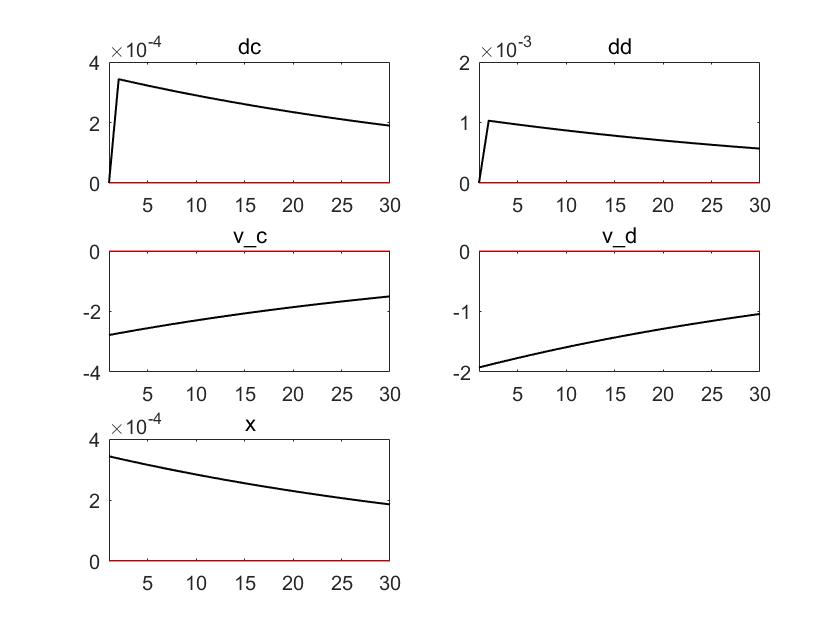
\includegraphics[width=0.8\linewidth]{fig34.jpg}
            \caption{Impulse response function to a shock to $x_t$ (CRRA preferences)}\label{34}
\end{figure}

\subsubsection{Epstein-Zin specification}

This section focuses on the more general Epstein-Zin setup. In particular, we allow both risk aversion and IES to be larger than one. $\Phi$	 and, via equation (50), $\theta$ are the only two parameters to differ between Table 13 and Table 15.

\begin{table}[h]
\centering\caption{parameter calibration.The value of $\theta$ is calibrated to satisfy equation (50).}\label{15}
\begin{tabular}{cc}
  \hline
  Parameter&Calibration\\
  \hline
  $Psi$&1.5\\
  $\theta$&-19.5\\
  $\gamma$&7.5\\
  $\delta$&0.99\\
  $\mu_c$&0.0015\\
  $\sigma_c$&0.0078\\
  $\mu_d$&0.0015\\
  $\lambda_{d,x}$&3\\
  $\sigma_d$&0.0351\\
  $\rho_x$&0.979\\
  $\sigma_x$&0.0003432\\
  \hline
  \end{tabular}
\end{table}

\vspace{3cm}

By running the Dynare program with the change in the calibration of $\Phi$	 and $\theta$, the policy functions for $v_c$ and $v_d$ change to:

$$v_{c,t}=104.209-1146.216(x_t-\overline{x})$$
$$v_{d,t}=104.209-8023.511(x_t-\overline{x})$$

Dynare computes policy and transition functions as reported in Table 16.

\begin{table}{h}
\centering
\caption{Policy and transition functions, CRRA calibration}\label{16}
\begin{tabular}{lccccc}
\hline
&$\Delta c$&$\Delta d$&$v_c$&$v_d$&x\\
Constant&0.0015&0.0015&104.209&104.209&0\\
x(-1)&1&3&1122.145&7855.017&0.979\\
$e_c$&1&0&0&0&0\\
$e_x$&0&0&1146.216&8023.511&1\\
$e_d$&0&1&0&0&0\\
\hline
\end{tabular}
\end{table}

Therefore, a shock to $x_t$ will now have a positive effect on price-dividend ratios. Separating risk aversion from intertemporal substitution and modelling both as greater than unity produces the effect of changing the sign of the impact of the forecastable part of consumption and dividend growth on price-dividend ratios. The IRF reported in Figure 32 stress this finding.

\begin{figure}[htbp!]
		\centering
			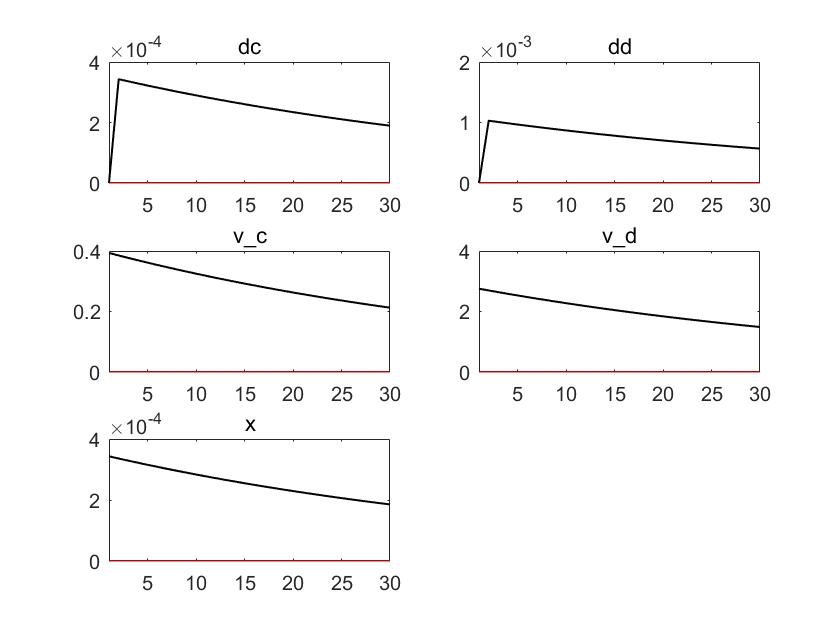
\includegraphics[width=0.8\linewidth]{fig35.jpg}
            \caption{Impulse response function to a shock to $x_t$ (Epstein-Zin preferences)}\label{35}
\end{figure}

\vspace{4cm}

\subsection{Bayesian estimation}

We perform a Bayesian estimation of the general model, using simulated series. The model has three shocks $\epsilon_c$,$\epsilon_x$ and $\epsilon_d$ and three observables $v_d, \Delta_c and \Delta_d$. The priors that we use are reported in Table 17. A slight modification to the program reported in the previous pages enables us to estimate the parameters of the model in Dynare. The following code was been used:\\
\\
\textcolor{blue}{
var  dc, dd, v\_c, v\_d, x;\\
varexo e\_c, e\_x, e\_d;
\\
parameters DELTA THETA PSI MU\_C MU\_D RHO\_X LAMBDA\_DX;\\
\\
DELTA=.99;\\
PSI=1.5;\\
THETA=(1-7.5)/(1-1/PSI);\\
MU\_C=0.0015;\\
MU\_D=0.0015;\\
RHO\_X=.979;\\
LAMBDA\_DX=3;\\
\\
model;
v\_c       = DELTA\^THETA * exp((-THETA/PSI)*dc(+1) + (THETA-1)*log((1+v\_c(+1))*exp(dc(+1))/v\_c) ) * (1+v\_c(+1))*exp(dc(+1));\\
v\_d       = DELTA\^THETA * exp((-THETA/PSI)*dc(+1) + (THETA-1)*log((1+v\_c(+1))*exp(dc(+1))/v\_c) ) * (1+v\_d(+1))*exp(dd(+1));\\
dc        = MU\_C  + x(-1) + e\_c;\\
dd        = MU\_D + LAMBDA\_DX*x(-1) + e\_d;\\
x         = RHO\_X * x(-1) + e\_x;\\
end;\\
\\
initval;\\
dc=MU\_C;\\
dd=MU\_D;\\
v\_c=DELTA*exp((1-1/PSI)*dc)/(1-DELTA*exp((1-1/PSI)*dc));\\
v\_d=(DELTA\^THETA*exp(-THETA/PSI*dc+dc*(THETA-1)+dd)*(1+v\_c)\^(THETA-1))\^(1/THETA);\\
x=0;\\
e\_c=0;\\
e\_x=0;\\
e\_d=0;\\
end;\\
\\
shocks;\\
var e\_d; stderr .001;\\
var e\_c; stderr .001;\\
var e\_x; stderr .001;\\
end;\\
\\\
steady;\\
\\
estimated\_params;\\
DELTA, beta\_pdf, 0.98,.005;\\
THETA,normal\_pdf,-19.5, 0.0025;\\
PSI,normal\_pdf,1.6, 0.1;\\
MU\_C,normal\_pdf,0.001, 0.001;\\
MU\_D,normal\_pdf,0.001, 0.001;\\
RHO\_X,normal\_pdf,.98, 0.005;\\
LAMBDA\_DX,normal\_pdf,3, 0.05;\\
stderr e\_d,inv\_gamma\_pdf,.0025, Inf;\\
stderr e\_x,inv\_gamma\_pdf,.0003, Inf;\\
stderr e\_c,inv\_gamma\_pdf,.01, Inf;\\
end;\\
\\
varobs v\_d dd dc;\\
\\
estimation(datafile=AssetPricing\_simuldata,mode\_compute=6,mh\_replic=1000,mh\_jscale=.4,nodiagnostic);}\\

In terms of Dynare’s output table 17 displays priors’ distributions, while Figure 33 reports a comparison between prior’s and posterior’s distributions. Since the data generating process is exactly the model that we are estimating, it is not very surprising that the distribution of the posterior has very little variance around the true parameters.

\begin{table}{h}
\centering
\caption{Priors}\label{17}
\begin{tabular}{lccc}
\hline
Parameter&Prior Distribution&Mean&Std.Dev.\\
\hline
$\Psi$&normal&1.5&0.005\\
$\theta$&normal&-19.5&0.005\\
$\delta$&beta&0.99&0.001\\
$\mu_c$&normal&0.0015&0.005\\
$\sigma_c$&Inv.Gamma&0.0078&inf.\\
$\mu_d$&normal&0.0015&0.005\\
$\lambda_{d,x}$&normal&3&0.05\\
$\sigma_d$&Inv.Gamma&0.0351&inf.\\
$\rho_x$&normal&0.979&0.05\\
$\sigma_x$&Inv.Gamma&0.0003432&inf.\\
\hline
\end{tabular}
\end{table}

Dynare also produces a table of summary statistics of the estimation. As already seen from the Figures, the mean of the posterior distributions is almost coincidental with the correct values and the estimated confidence interval is very tight around these values. Table 18 reports these numbers.

\begin{table}{h}
\centering
\caption{Priors and Posteriors}\label{18}
\begin{tabular}{lcccccc}
\hline
Parameter&Prior Mean&Post.Mean&90\% HPD&Interval&Prior Dis.&Post.Std.Dev.\\
\hline
$\Psi$&1.6&1.5824&1.5428&1.6120&normal&0.1\\
$\theta$&-19.5&-19.4996&-19.5006&-19.4987&normal&0.0025\\
$\delta$&0.98&0.9892&0.9884&0.9898&beta&0.005\\
$\mu_c$&0.001&0.0011&0.0008&0.0015&normal&0.001\\
$\sigma_c$&0.01&0.0079&0.0075&0.0081&Inv.Gamma&inf.\\
$\mu_d$&0.001&0.002&0.0012&0.0025&normal&0.001\\
$\lambda_{d,x}$&3&2.9943&2.9736&3.0154&normal&0.05\\
$\sigma_d$&0.003&0.0347&0.0335&0.0360&Inv.Gamma&inf.\\
$\rho_x$&0.980&0.9805&0.9787&0.9823&normal&0.005\\
$\sigma_x$&0.000&0.0003&0.0003&0.0004&Inv.Gamma&inf.\\
\hline
\end{tabular}
\end{table}

\begin{figure}[htbp!]
		\centering
			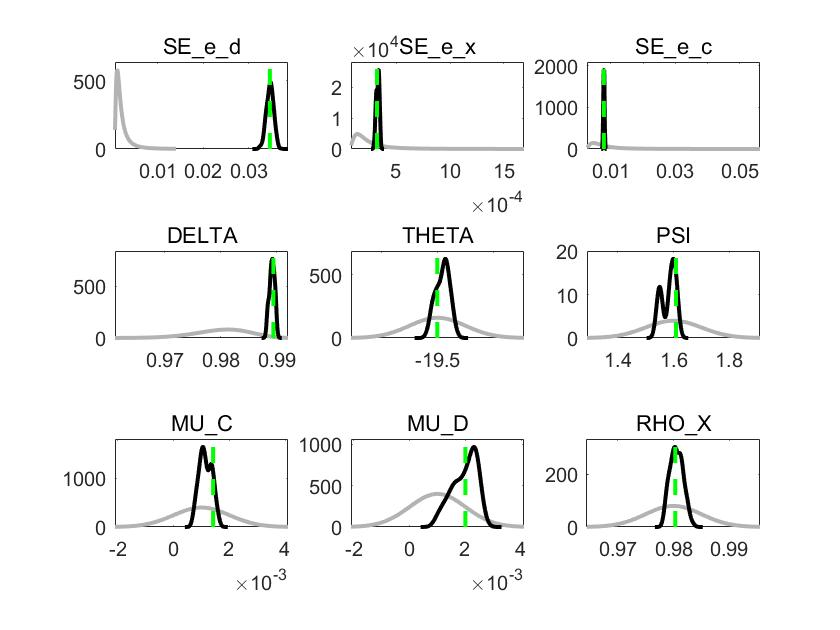
\includegraphics[width=0.8\linewidth]{fig36.jpg}
            \caption{Posterior)}\label{36}
\end{figure}


%_________________ End of Main Matter_________________%

\clearpage

%_________________ Reference Section _______________%

\phantomsection                                   % allows for correct link to Table of Contents
%\addcontentsline{toc}{section}{References}        % Adds the line "References" to Table of contents
\onehalfspacing


\printbibliography % print the bibliography using BibLaTex
\section{References}
Bansal, R., R. Gallant, and G. Tauchen (2007). Rational pessimism, rational exuberance and markets for macro risks. Working Paper .\\

Bansal, R. and A. Yaron (2004, 08). Risks for the long run: A potential resolution of asset pricing puzzles. Journal of Finance 59(4), 1481–1509.\\

Burnside, C. (1998, March). Solving asset pricing models with gaussian shocks. Journal of Economic Dynamics and Control 22(3), 329–340.\\

Cagan, P. (1956). The monetary dynamics of hyperinflation. In M. Friedman (Ed.), Studies in the Quantity Theory of Money. University of Chicago Press.\\

Cooley, T. F. and E. C. Prescott (1995). Economic growth and business cycles. In T. F. Cooley (Ed.), Frontiers of Business Cycle Research. Princeton University Press.\\

Epstein, L. G. and S. E. Zin (1989, July). Substitution, risk aversion, and the temporal behavior of consumption and asset returns: A theoretical framework. Econometrica 57(4), 937–69.\\

Epstein, L. G. and S. E. Zin (1991, April). Substitution, risk aversion, and the temporal behavior of consumption and asset returns: An empirical analysis. Journal of Political Economy 99(2), 263–86.\\

Hall, R. E. (1988, April). Intertemporal substitution in consumption. Journal of Political Economy 96(2), 339–57.\\

Hansen, L. P., T. J. Sargent, and J. Tallarini, Thomas D (1999, October). Robust permanent income and pricing. Review of Economic Studies 66(4), 873–907.\\

Kim, J. and S. H. Kim (2003, August). Spurious welfare reversals in international business cycle models. Journal of International Economics 60(2), 471–500.\\

Ljungqvist, L. and T. J. Sargent (2004). Recursive Macroeconomic Theory, Second edition. Cambridge, Ma.: MIT Press.\\

Ljungqvist, L. and T. J. Sargent (20XX). Recursive Macroeconomic Theory, Third edition. Cambridge, Ma.: MIT Press.\\

Ryoo, J. and S. Rosen (2004, February). The engineering labor market. Journal of Political Economy 112(S1), S110–S140.\\

Sargent, T. J. (1977, February). The demand for money during hyperinflations under rational expectations: I. International Economic Review 18 (1), 59–82.\\

Schmitt-Grohe, S. and M. Uribe (2004). Solving asset pricing models with gaussian shocks. Journal of Economic Dynamics and Control 28, 755–775.\\

Slow, A. (1984, May). Occupational choice under uncertainty. Econometrica 52(3), 631–45.

%% alternative using BibTeX
%\bibliographystyle{econometrica}                  % sets the style for the Bibliography
%\bibliography{mybibfile}                         % Uses the Bibtex-file mybibfile.bib


\clearpage
%_________________ Space for Supplementary Material _______________%
\appendix
\numberwithin{equation}{section} %restarts equation numbering with 1 and adds the appendix in front
\numberwithin{table}{section} %same for Tables
\numberwithin{figure}{section} %and for Figures

\section{Appendix List of Dynare Files}

This appendix lists the dynare files used in this paper. All files and the data used are contained in the file examples2019.zip. In case simulated data was used in the estimation one first needs to run the relevant dynare code to simulate the data.
\begin{itemize}
  \item neoclassical\_growth\_model.mod - solves the neoclassical growth model and simulates data;
\item neoclassical\_growth\_model\_est.mod - estimates the neoclassical growth model
\item international\_BC.mod - solves the two country production economy and simulates data
\item international\_BC\_est.mod - estimates the two country production economy
\item neoclassical\_fiscal\_figX.mod - solves a deterministic growth model and reproduces the graph in chapter 11 of Ljungqvist and Sargent (2004)
\item sargent77.mod - solves the model in Sargent (1977)
\item sargent77ML.mod, sargent77Bayes.mod - estimate the model in Sargent (1977) using maximum likelihood and Bayesian MCMC methods, respectively
\item hall1.mod - solves the model in Hall (1988) and simulates data
\item hall1estimateML.mod, hall1estimateBayes.mod - estimate the model in Hall (1988) using maximum likelihood and Bayesian MCMC methods, respectively
\item rosen.mod - solves the model in Ryoo and Rosen (2004) and simulates data
  \item rosenestimateML.mod, rosenestimateBayes.mod - estimate the model in Ryoo and Rosen (2004) using maximum likelihood and Bayesian MCMC methods, respectively
\item BansalYaronML.mod, BansalYaronBayes.mod - estimate the consumption-growth process of Bansal and Yaron (2004) using maximum likelihood and Bayesian MCMC methods, respectively
\item HSTML.mod, HSTBayes.mod - estimate the model in Hansen, Sargent, and Tallarini (1999) using maximum likelihood and Bayesian MCMC methods, respectively
\item AssetPricingApproximation.mod - solves the model of Bansal and Yaron (2004) and simulates data
\item AssetPricingEstimate.mod - estimates the model of Bansal and Yaron (2004)
\end{itemize}


\end{document}
